% -*- Mode:TeX -*-

%% IMPORTANT: The official thesis specifications are available at:
%%            http://libraries.mit.edu/archives/thesis-specs/
%%
%%            Please verify your thesis' formatting and copyright
%%            assignment before submission. If you notice any
%%            discrepancies between these templates and the 
%%            MIT Libraries' specs, please let us know
%%            by e-mailing thesis@mit.edu

%% The documentclass options along with the pagestyle can be used to generate
%% a technical report, a draft copy, or a regular thesis. You may need to
%% re-specify the pagestyle after you \include cover.tex. For more
%% information, see the first few lines of tfm.cls. 

%\documentclass[12pt,vi,twoside]{tfm}
%%
%%  If you want your thesis copyright to you instead of MIT, use the
%%  ``vi'' option, as above.
%%
%\documentclass[12pt,twoside,leftblank]{tfm}
%%
%% If you want blank pages before new chapters to be labelled ``This
%% Page Intentionally Left Blank'', use the ``leftblank'' option, as
%% above.

\documentclass[12pt, oneside]{tfm}
\usepackage{lgrind}
\usepackage{cmap}
\usepackage[T1]{fontenc}
\pagestyle{plain}

% Cover packages/commands
\usepackage{afterpage}
\usepackage{graphicx}
\usepackage{contour}
\pagenumbering{gobble}

% Bibliography packages/commands
\usepackage{IEEEtrantools}
\usepackage[colorlinks=true, linkcolor=black, urlcolor=black,  citecolor=black]{hyperref}
\renewcommand{\bibname}{References}
\usepackage{notoccite}

% List/Sublist
\usepackage{outlines}

% Figures
\usepackage{caption}
\usepackage{subcaption}
\captionsetup[figure]{labelfont={bf}, labelsep={period}}

% Tables
\usepackage{longtable}
\usepackage{multirow}
\usepackage[table]{xcolor} % xcolor package is also used for the cover
\usepackage{enumitem}
\captionsetup[table]{labelfont={bf}, labelsep={period}}

% Copyright
\usepackage{textcomp}

% Chemistry package
\usepackage[version=4]{mhchem}

% Remove hyphenation
% \tolerance=1
% \emergencystretch=\maxdimen
% \hyphenpenalty=10000
% \hbadness=10000

%% This bit allows you to either specify only the files which you wish to
%% process, or `all' to process all files which you \include.
%% Krishna Sethuraman (1990).

%\typein [\files]{Enter file names to process, (chap1,chap2 ...), or `all' to process all files:}
\def\all{all}
\ifx\files\all \typeout{Including all files.} \else %\typeout{Including only \files.} \includeonly{\files} \fi

\begin{document}
    \bstctlcite{BSTcontrol} % Max bibtex authors
    \definecolor{orange}{RGB}{253,178,132}
\definecolor{orange2}{RGB}{239,104,31}
\definecolor{grey}{RGB}{128,128,128}
\pagecolor{orange}\afterpage{\nopagecolor}
\begin{center}
    \contour{black}{\LARGE{\textbf{UNIVERSIDAD POLITÉCNICA DE MADRID}}} \\
    \vspace{1cm}
    {\Large{ESCUELA TÉCNICA SUPERIOR \\ DE INGENIEROS DE TELECOMUNICACIÓN}} \\
    \vspace{1cm}
    
\includegraphics[width=8cm,height=2.2cm]{Images/covers/Logo_ETSIT_1.png} \\
    \vspace{1cm}
    {\Large{MASTER OF SCIENCE IN \\ BIOMEDICAL ENGINEERING}} \\
    \vspace{3cm}
    \contour{black}{\LARGE{\textbf{MASTER's THESIS}}} \\
    \vspace{1.2cm}
    \contour{orange}{\Large{\textsc{\textbf{DEVELOPMENT OF A BIOINFORMATIC}}}} \\ 
    \contour{orange}{\Large{\textsc{\textbf{PIPELINE FOR THE DETECTION OF}}}} \\
    \contour{orange}{\Large{\textsc{\textbf{SOMATIC MUTATIONS IN LIQUID BIOPSY}}}} \\
    \contour{orange}{\Large{\textsc{\textbf{SAMPLES FROM NON-SMALL CELL}}}} \\
    \contour{orange}{\Large{\textsc{\textbf{LUNG CANCER PATIENTS}}}} \\
    \vspace{2cm}
    {\large{VADYM IVANCHUK}} \\
    \vspace{0.1cm}
    {\large{2020}}
\end{center}
    \newpage\null\thispagestyle{empty}\newpage
    \begin{titlepage}
\begin{large}
    \textbf{MASTER's THESIS}
        \signature{\break}{}
        \signature{Title}{\textit{Development of a bioinformatic pipeline for the \\ detection of somatic mutations in liquid biopsy \\ samples from non-small cell lung cancer patients}}
        \signature{Author}{\textit{Vadym Ivanchuk}}
        \signature{Supervisor}{\textit{Atocha Romero Alfonso \\ Estela Sánchez Herrero}}
        \signature{Tenured professor}{\textit{Milagros Ramos Gomez}}
        \signature{Department}{\textit{Tecnología Fotónica y Bioingeniería}}
        \signature{\break}{}
    \textbf{COURT}
        \signature{\break}{}
        \signature{President}{\textit{}}
        \signature{Vocal}{\textit{}}
        \signature{Secretary}{\textit{}}
        \signature{Substitute}{\textit{}}
        \signature{\break}{}
    \hspace*{2.05cm}\begin{tabular}{c | c}
        \textbf{DATE} & \\
    \end{tabular}
    \newline \break
    \hspace*{-1.93cm}\begin{tabular}{c | c}
        \textbf{GRADE} & \\
    \end{tabular}
\end{large}
\end{titlepage}

    \newpage\null\thispagestyle{empty}\newpage
    \begin{center}
    \contour{black}{\LARGE{\textbf{UNIVERSIDAD POLITÉCNICA DE MADRID}}} \\
    \vspace{1cm}
    {\Large{ESCUELA TÉCNICA SUPERIOR \\ DE INGENIEROS DE TELECOMUNICACIÓN}} \\
    \vspace{1cm}
    
\includegraphics[width=8cm,height=2.2cm]{Images/covers/Logo_ETSIT_2.png} \\
    \vspace{1cm}
    {\Large{MASTER OF SCIENCE IN \\ BIOMEDICAL ENGINEERING}} \\
    \vspace{3cm}
    \contour{black}{\LARGE{\textbf{MASTER's THESIS}}} \\
    \vspace{1.2cm}
    \contour{white}{\Large{\textsc{\textbf{DEVELOPMENT OF A BIOINFORMATIC}}}} \\ 
    \contour{white}{\Large{\textsc{\textbf{PIPELINE FOR THE DETECTION OF}}}} \\
    \contour{white}{\Large{\textsc{\textbf{SOMATIC MUTATIONS IN LIQUID BIOPSY}}}} \\
    \contour{white}{\Large{\textsc{\textbf{SAMPLES FROM NON-SMALL CELL}}}} \\
    \contour{white}{\Large{\textsc{\textbf{LUNG CANCER PATIENTS}}}} \\
    \vspace{2cm}
    {\large{VADYM IVANCHUK}} \\
    \vspace{0.1cm}
    {\large{2020}}
\end{center}
    \newpage\null\thispagestyle{empty}\newpage
    \pagenumbering{roman}
    %\chapter*{Acknowledgments}
\addcontentsline{toc}{chapter}{Acknowledgments}  

Bla bla bla bla ...

    %\afterpage{\null\newpage}
    \chapter*{Abstract}
\addcontentsline{toc}{chapter}{Abstract}

...

\begingroup % Multiple chapters in the same page
\renewcommand{\cleardoublepage}{}
\renewcommand{\clearpage}{}
\chapter*{Keywords}
\endgroup

...

    \afterpage{\null\newpage}
    \chapter*{Glossary}
\addcontentsline{toc}{chapter}{Glossary}

\footnotesize
\begin{longtable}[l]{l l}
    \textbf{AKT} & Protein Kinase B \\ 
    \textbf{ALCL} & Anaplastic Large-Cell Lymphoma \\
    \textbf{ALK} & Anaplastic Lymphoma Kinase \\
    \textbf{AMP} & Association of Molecular Pathologists \\
    \textbf{BBB} & Blood-Brain Barrier \\
    \textbf{BRAF} & V-Raf Murine Sarcoma Viral Oncogene Homolog B1 \\
    \textbf{CAP} & College of American Pathologists \\
    \textbf{cDNA} & Complementary DNA \\
    \textbf{cfDNA} & Circulating Free DNA \\
    \textbf{CNS} & Central Nervous System \\
    \textbf{CNV} & Copy Number Variation \\
    \textbf{CTC} & Circulating Tumor Cell \\
    \textbf{ctDNA} & Circulating Tumor DNA \\
    \textbf{CTLA-4} & Cytotoxic T-Lymphocyte-Associated Antigen 4 \\
    \textbf{DNA} & Deoxyribonucleic Acid \\
    \textbf{dNTP} & Deoxyribonucleotide Triphosphate \\
    \textbf{dPCR} & Digital PCR \\
    \textbf{ECOG} & Eastern Cooperative Oncology Group \\
    \textbf{EGFR} & Epidermal Growth Factor Receptor \\
    \textbf{EMA} & European Medicines Agency \\
    \textbf{EML4} & Echinoderm Microtubule-Associated Protein-Like 4 \\
    \textbf{EMT} & Epithelial–Mesenchymal Transition \\
    \textbf{EpCAM} & Epithelial Cell Adhesion Molecule \\
    \textbf{ePCR} & Emulsion PCR \\
    \textbf{ERK} & Extracellular Signal Regulated Kinase \\
    \textbf{ERRB} & Avian Erythroblastosis Oncogene B \\
    % \textbf{EV} & Extracellular Vesicle \\
    \textbf{FDA} & Food and Drug Administration \\
    \textbf{FGF} & Fibroblast Growth Factor \\
    \textbf{FISH} & Fluorescence in Situ Hybridization \\
    \textbf{GCO} & Global Cancer Observatory \\
    \textbf{HER2} & Human Epidermal Growth Factor Receptor 2 \\
    \textbf{IASLC} & International Association for the Study of Lung Cancer \\
    \textbf{IGF-1R} & Insulin-Like Growth Factor 1 Receptor \\
    \textbf{IGV} & Integrative Genomics Viewer \\
    \textbf{IHC} & Immunohistochemistry \\
    \textbf{InDel} & Insertions and Deletion \\
    \textbf{JAK} & Janus Kinase \\
    \textbf{KRAS} & Kirsten Rat Sarcoma \\
    \textbf{LOD} & Limit of Detection \\
    \textbf{MAPK} & Mitogen-Activated Protein Kinase \\
    \textbf{MEK} & Mitogen Activated Protein Kinase \\
    \textbf{MET} & Mesenchymal–Epithelial Transition \\
    \textbf{mRNA} & Messenger RNA \\
    \textbf{mTOR} & Mammalian Target of Rapamycin \\
    \textbf{NGS} & Next-Generation Sequencing \\
    \textbf{NPM} & Nucleophosmin \\
    \textbf{NRG1} & Neuregulin 1 \\
    \textbf{NSCLC} & Non-Small Cell Lung Cancer \\
    \textbf{NTRK1} & Neurotrophic Tyrosine Kinase Receptor 1 \\
    \textbf{ORR} &  Overall Response Rate \\
    \textbf{OS} & Overall Survival \\
    \textbf{PCR} & Polymerase Chain Reaction \\
    \textbf{PD-1} & Programmed Cell Death Protein 1 \\
    \textbf{PD-L1} & Programmed Death-Ligand 1 \\
    \textbf{PDGF} & Platelet-Derived Growth Factor \\
    \textbf{PFS} & Progression-Free Survival \\
    \textbf{PI3K} & Phosphoinositide 3-Kinase \\
    \textbf{qPCR} & Quantitative PCR \\
    \textbf{RAF} & Rapidly Accelerated Fibrosarcoma \\
    \textbf{RAS} & Rat Sarcoma \\
    \textbf{RET} & Rearranged During Transfection \\
    \textbf{RNA} & Ribonucleic Acid \\
    \textbf{ROS} & Reactive Oxygen Species \\
    \textbf{ROS1} & Reactive Oxygen Species Proto-Oncogene 1 \\
    \textbf{RR} & Response Rate \\
    \textbf{RT-PCR} & Reverse Transcription PCR \\
    \textbf{SCLC} & Small Cell Lung Cancer \\
    \textbf{SNV} & Single Nucleotide Variant \\
    \textbf{STAT} & Signal Transducer and Activator of Transcription Proteins \\
    \textbf{TEP} & Tumor-Educated Platelet \\
    \textbf{TKI} & Tyrosine Kinase Inhibitor \\
    \textbf{VATS} & Video-Assisted Thoracoscopic Surgery \\
    \textbf{VEGF} & Vascular Endothelial Growth Factor \\
    \textbf{VEGFR} & Vascular Endothelial Growth Factor Receptor \\
\end{longtable}

\normalsize

    \afterpage{\null\newpage}
      % -*- Mode:TeX -*-
%% This file simply contains the commands that actually generate the table of
%% contents and lists of figures and tables.  You can omit any or all of
%% these files by simply taking out the appropriate command.  For more
%% information on these files, see appendix C.3.3 of the LaTeX manual.
\tableofcontents
\newpage
\listoffigures
\addcontentsline{toc}{chapter}{List of Figures}
\newpage
\phantomsection
\addcontentsline{toc}{chapter}{List of Tables}\listoftables

    \newpage\null\newpage
    \setcounter{page}{0}
    \pagenumbering{arabic}
    \chapter{Introduction}

\section{Cancer}

\subsection{Background}

Cancer is a very broad term that covers more than 200 types of diseases \cite{WCR}. Each of them can have completely different characteristics from each other and can be considered as independent diseases with their causes, evolution, and specific treatments. However, they all have a common denominator: cancer cells acquire the ability to multiply and spread throughout the body without control.

Cancer arises from the transformation of normal cells into tumor cells in a process that could be divided into at least four consecutive stages \cite{Stages}: initiation, promotion, progression, and metastasis (\autoref{fig:Carcinogenesis}). Initiation involves the alteration, change, or mutation of genes arising spontaneously or induced by exposure to a carcinogenic agent. The promotion stage is considered to be a relatively lengthy and reversible process in which actively proliferating preneoplastic cells accumulate, while progression is the phase between a premalignant lesion and the development of invasive cancer. Progression is the final stage of neoplastic transformation, where the cells may undergo further genetic and phenotypic changes with invasive and metastatic potential. Finally, metastasis, which is responsible for as much as 90\% of cancer-associated mortality \cite{Metastasis}, involves the spread of cancer cells from the primary site to other parts of the body through the bloodstream or the lymph system.

\begin{figure}[t]
    \centering
    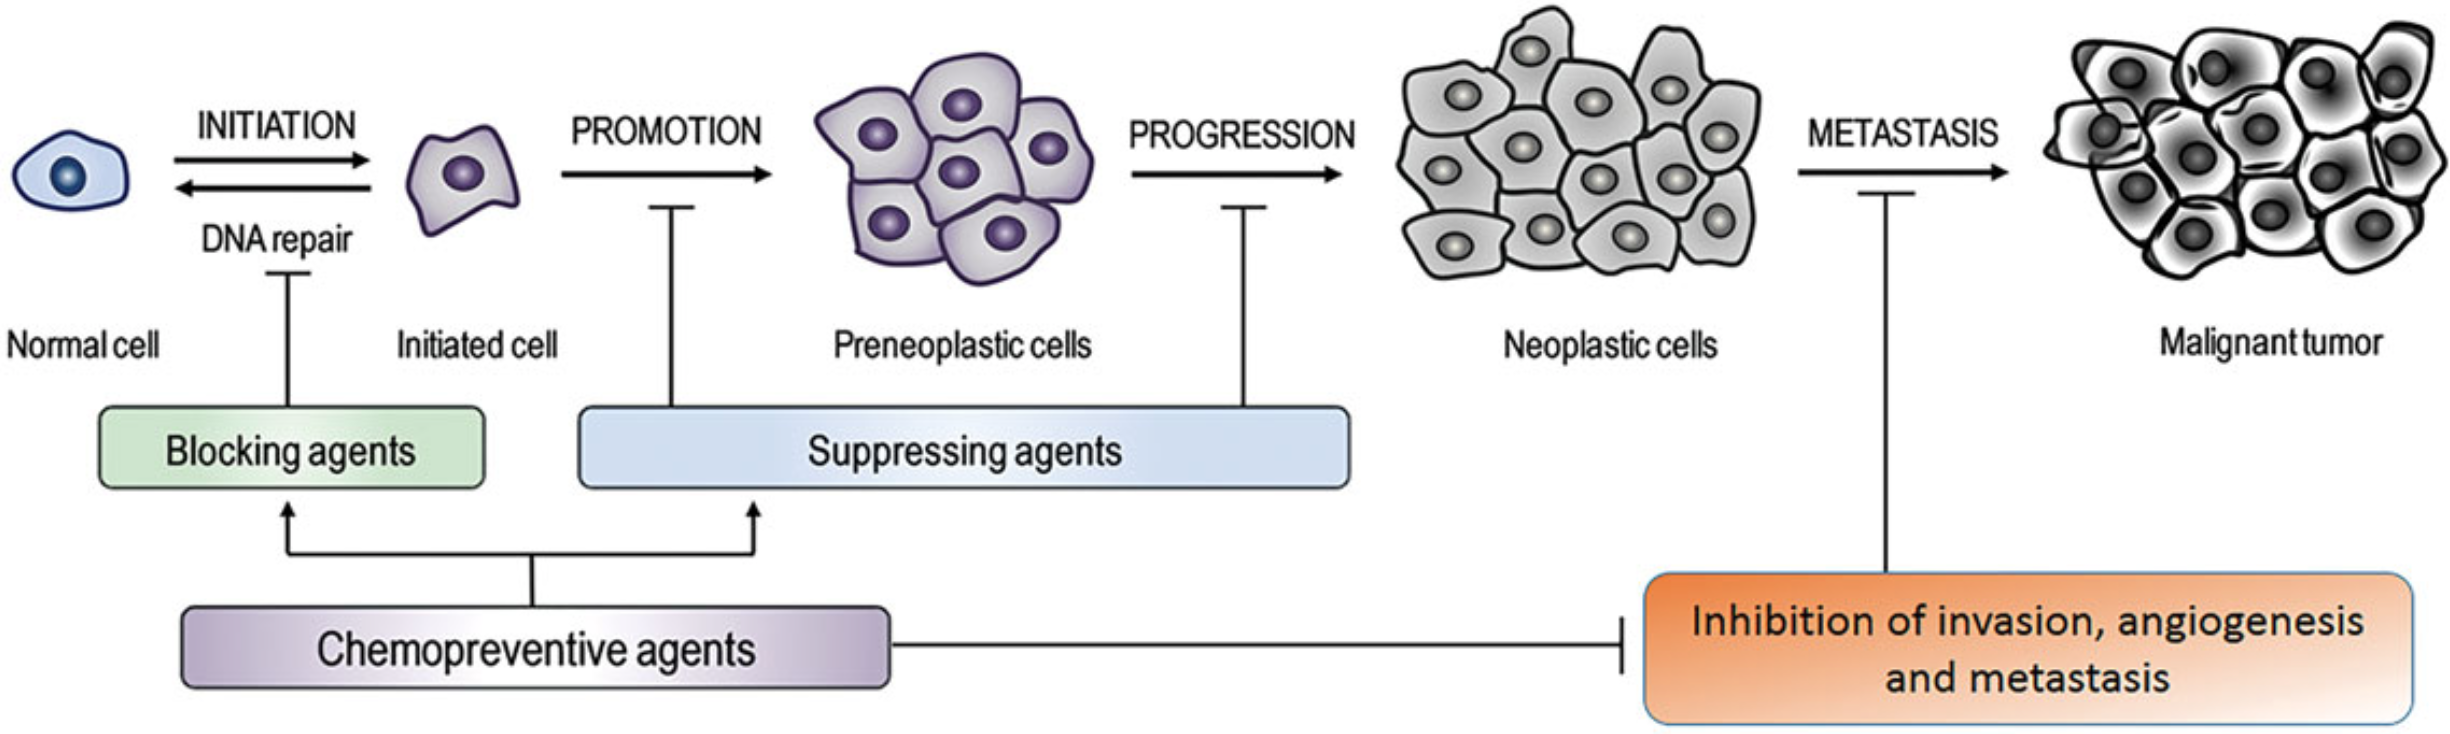
\includegraphics[width=\textwidth]{Images/chapter_1/carcinogenesis.png}
    \caption{Carcinogenesis phases: initiation, promotion, progression, and metastasis. Modified image from \cite{Stages}.}
    \label{fig:Carcinogenesis}
\end{figure}

During this multi-step development of tumors, cancer cells acquire some biological capabilities that are considered the hallmarks of cancer \cite{Hallmarks}. They include sustaining proliferative signaling, evading growth suppressors, resisting cell death, enabling replicative immortality, inducing angiogenesis, activating invasion and metastasis, reprogramming of energy metabolism, and evading immune destruction. Furthermore, underlying these hallmarks are genome instability, which generates the genetic diversity that expedites their acquisition and inflammation, which fosters multiple hallmark functions. All these characteristics constitute an organizing principle to rationalize the complexities of this neoplastic disease and are widely recognized and applicable in cancer treatments, especially in targeted therapies.

These biological changes in normal cells are primarily the result of the interaction between a person's genetic factors and 3 categories of external agents \cite{WCR}, including physical carcinogens (ultraviolet and ionizing radiation), chemical carcinogens (asbestos, components of tobacco smoke, etc.) and biological carcinogens (infections from certain viruses, bacteria or parasites). Aging is another fundamental factor for the development of cancer since its incidence rises dramatically with age \cite{Globocan}.

Finally, the magnitude of this problem is reflected by the Global Cancer Observatory (GCO) \cite{Globocan} in the fact that this pathology is the leading cause of death worldwide, accounting for an estimated 9.6 million deaths in 2018. Furthermore, every year about 18.1 million new cases are diagnosed, being the lung and breast cancers the most common types with a joint incidence of 23.2\% (\autoref{fig:GCO_1}). However, when it comes to mortality, lung cancer stands out above the rest with 1.76 million deaths, doubling even the numbers of the second most lethal cancer, the colorectal (\autoref{fig:GCO_2}).

\begin{figure}[t]
    \centering
    \begin{subfigure}{0.49\textwidth}
        \centering
        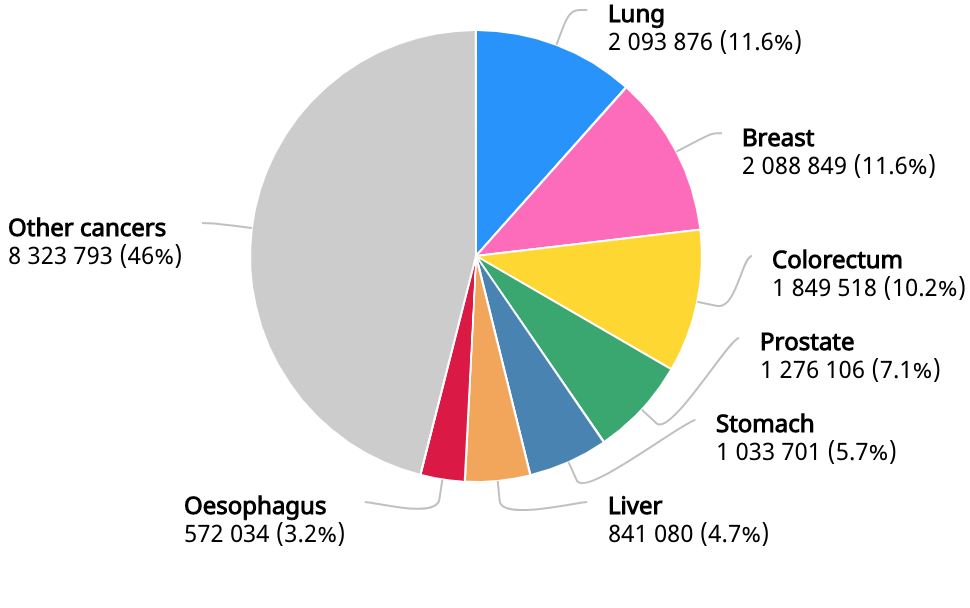
\includegraphics[width=\textwidth]{Images/chapter_1/cancer_cases.png}
        \caption{Number of new cases.}
        \label{fig:GCO_1}
    \end{subfigure}
    \hfill
    \begin{subfigure}{0.49\textwidth}
        \centering
        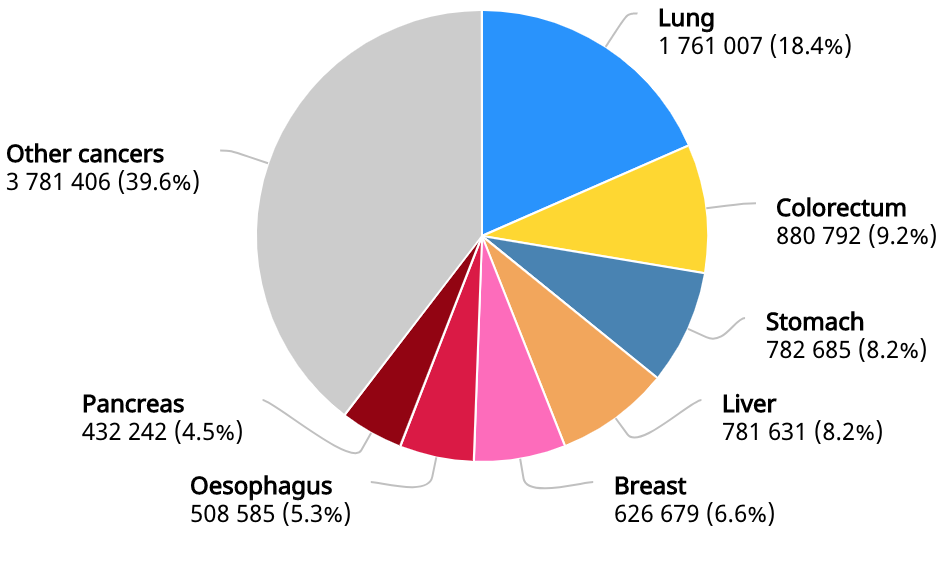
\includegraphics[width=\textwidth]{Images/chapter_1/cancer_deaths.png}
        \caption{Number of deaths.}
        \label{fig:GCO_2}
    \end{subfigure}
    \caption{Cancer incidence and mortality statistics worldwide in 2018. Images from \cite{GCO}.}
    \label{fig:GCO}
\end{figure}

\subsection{Lung Cancer}

Lung cancer is a group of diseases resulting from the malignant growth of cells of the respiratory tract, in particular of the lining epithelium of the bronchi, bronchioles, or alveoli. In the last century, it has progressed from an uncommon disease to the most prevalent cancer in the world and the most common cause of death from cancer. Its mortality is very close to its incidence since only 20.5\% of people are still alive 5 years after being diagnosed in the United States \cite{SEER}. Furthermore, according to a population-based study of lung cancer survival and stage at diagnosis worldwide \cite{Walters}, only 15–20\% of cases are diagnosed when the tumor can be removed by surgical resection. In 20-25\% of people, the neoplasm is detected when it has a regional extension and can still be cured by combined chemotherapy and radiation therapy techniques. However, in 55–65\% of cases, this type of cancer is diagnosed at an advanced stage when only palliative care treatments or participation in clinical trials are considered, which are focused on treating the symptoms rather than cancer itself.

This progressive tumor development, which dramatically decreases patients' survival \cite{SEER}, can spread and proliferate in three main ways:
\begin{itemize}
    \item \textbf{Local growth}, which can eventually lead to an invasion through the lung walls of some of the surrounding structures, such as the heart, great vessels, esophagus, or vertebral bodies, depending on the initial location of the neoplasm.
    \item \textbf{Lymphatic dissemination}. It is done through the lymph. The presence of tumors in the middle and lower third of the lungs tend to proliferate mainly to the mediastinal lymph nodes, whereas tumors in the upper third are more likely to affect the supraclavicular lymph nodes.
    \item \textbf{Hematogenous dissemination}. The propagation of tumor cells is carried out through the blood vessels and can potentially affect the liver, adrenal glands, brain, and bones.
\end{itemize}

%\begin{figure}[t]
%    \centering
%    \begin{subfigure}{0.55\textwidth}
%        \centering
%        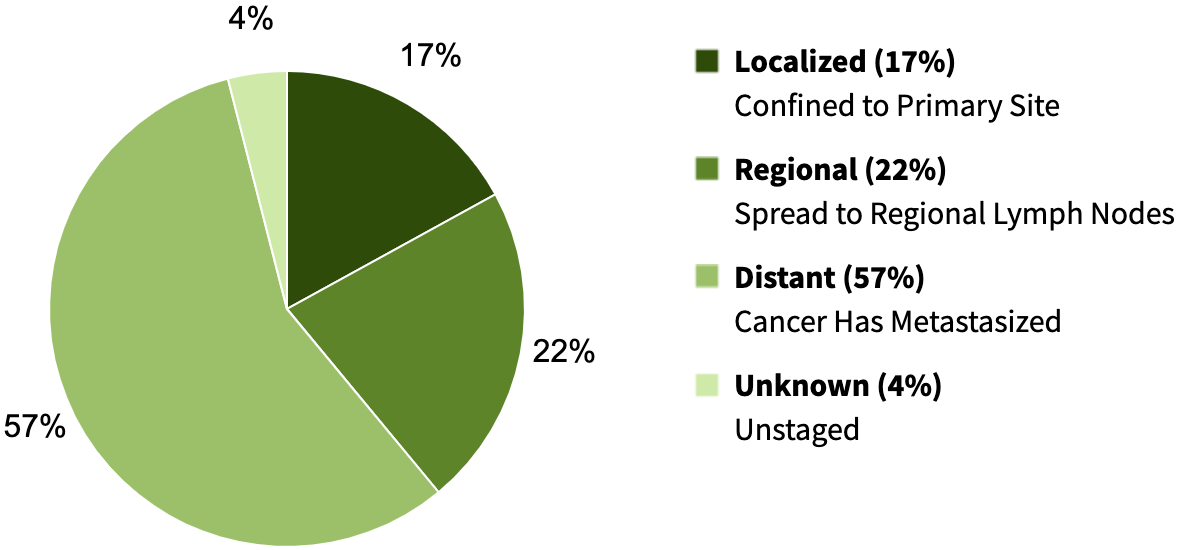
\includegraphics[width=\textwidth]{Images/chapter_1/cases_by_stage.png}
%        \caption{Percent of cases by stage.}
%        \label{fig:SEER_1}
%    \end{subfigure}
%    \hfill
%    \begin{subfigure}{0.44\textwidth}
%        \centering
%        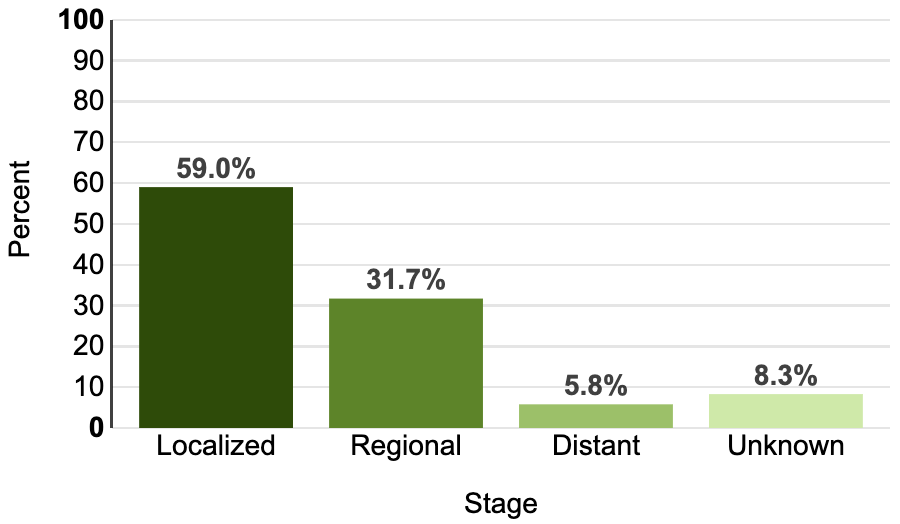
\includegraphics[width=\textwidth]{Images/chapter_1/5_year_survival.png}
%        \caption{5-year relative survival.}
%        \label{fig:SEER_2}
%    \end{subfigure}
%    \caption{Percent of cases and 5-year relative survival by stage at diagnosis between 2010 and 2016 \cite{SEER}.}
%    \label{fig:SEER}
%\end{figure}

To diagnose lung cancer and determine whether it has spread to other parts of the body, many different tests are used and some of them can also help to decide which treatments might work best. The steps to make an effective diagnosis usually include studying the patients' medical history, laboratory tests, imaging tests, biopsies, and biomarker tests. However, currently, only a biopsy can provide a definite diagnosis of lung cancer.

In this way and as a previous step to treatment, it is essential to make an accurate histological diagnosis of the tumor as each one of its types presents a different natural evolution. Therefore, the most common forms of lung cancer are classified according to the characteristics of the cells from which they are derived \cite{WHO}, distinguishing two large groups:
\begin{itemize}
    \item \textbf{Small cell lung cancer (SCLC)}. It is a very aggressive malignant neoplasm that accounts for about 15\% of lung cancer cases \cite{SCLC} and is characterized by a rapid doubling time, high growth ratio, and a greater propensity for early development of widespread metastases. The origin of SCLC tumor cells has not been formally identified, although they are commonly thought to arise from neuroendocrine cells in the bronchus \cite{SCLC_cell_orig}. Finally, this neoplasm has been described mainly in the elderly with a history of long exposure to tobacco.
    \item \textbf{Non-small cell lung cancer (NSCLC)}. It is the most common type of lung cancer, accounting for approximately 85\% of all cases, and it is the most common form in women, young adults, and people who haven't smoked \cite{NSCLC}. Furthermore, this histological subtype of lung cancer is not as lethal as SCLC, since it usually grows and spreads more slowly and can, therefore, be detected at less advanced stages. In this sense, depending on the staging, this type of patients are often eligible for a wider variety of treatments ranging from surgery to radiation, chemotherapy as well as targeted therapy.
\end{itemize}

Finally, despite the severity of this disease, it is largely preventable since there is a close relationship between the amount of exposure to tobacco carcinogens and the subsequent appearance of lung cancers several years or decades later \cite{Tobacco}. It is estimated that tobacco smoking explains almost 90\% of lung cancer risk in men and 70–80\% in women \cite{Smoking}.

\section{Non-Small Cell Lung Cancer (NSCLC)}

\subsection{Histological Classification}

There are three major types of non-small cell lung cancer:
\begin{itemize}
    \item \textbf{Squamous-cell carcinoma}, which comprises 25–30\% of all NSCLC cases \cite{NSCLC}. It arises from early versions of squamous cells in the airway epithelial cells in the central part of the lungs, that is, in the bronchi. Therefore, squamous cell carcinoma tends to cause symptoms earlier since it affects the larger airways of the lungs. On the other hand, although this type of cancer is generally slow-growing, it has the potential to spread to multiple sites due to its initial location, including the brain, spine and other bones, adrenal glands, and liver \cite{NSCLC_metastases}. In addition, this subtype is strongly correlated with cigarette smoking, more than any other form of NSCLC \cite{Tobacco, Smoking}.
    \item \textbf{Adenocarcinoma}. It is the most common type of lung cancer, accounting for approximately 40\% of NSCLC \cite{NSCLC}. Compared to the other forms, it tends to grow more slowly and has a greater chance of being found before spreading outside the lungs. It usually starts in glandular cells, which secrete mucus and other substances, and tends to develop in smaller airways, such as alveoli. Additionally, it is normally located more along the outer edges of the lungs and as a result, it frequently affects the pleura and chest wall \cite{ALA}. Currently, it is not only the most common type in smokers, but it is also the most common form of lung cancer in women, Asians, and people under the age of 45 \cite{AD_survival}. Finally, in recent years, this histological variant has gained special interest with the discovery of a series of molecular alterations in a subgroup of patients that is allowing them to be treated with targeted therapies \cite{AD_savini}.
    \item \textbf{Large cell (undifferentiated) carcinoma}. It accounts for 5–10\% of lung cancers \cite{NSCLC}. However, as more exact ways of diagnosing lung cancer have come into use, many tumors, previously labeled as undifferentiated large cell carcinoma, can now be classified more appropriately as poorly differentiated adenocarcinoma or squamous cell carcinoma \cite{LCC}. For this reason, the incidence of this type of tumor continues to decrease and it is often diagnosed by default through the exclusion of other possibilities and where is no evidence of squamous or glandular maturation. It usually begins in the epithelial cells on the outer edges of the lungs and tends to grow and spread rapidly \cite{LCC_bio}, which can make it harder to treat. Furthermore, and as in the other types, it is concluded that cigarette smoking is the predominant cause of large cell lung cancer \cite{LCC_smoking}.
\end{itemize}

%\begin{figure}[t]
%    \centering
%    \begin{subfigure}{0.4\textwidth}
%        \centering
%        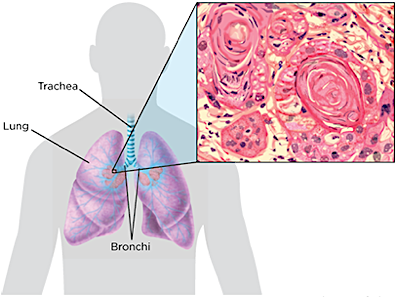
\includegraphics[width=\textwidth]{Images/chapter_1/squamous.png}
%        \caption{Squamous-cell carcinoma.}
%        \label{fig:squamous}
%    \end{subfigure}
%    \hfill
%    \begin{subfigure}{0.4\textwidth}
%        \centering
%        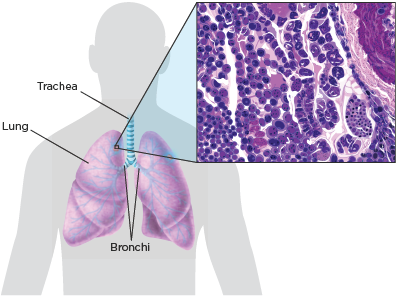
\includegraphics[width=\textwidth]{Images/chapter_1/adenocarcinoma.png}
%        \caption{Adenocarcinoma.}
%        \label{fig:adeno}
%    \end{subfigure}
%    \hfill
%    \begin{subfigure}{0.4\textwidth}
%    \centering
%    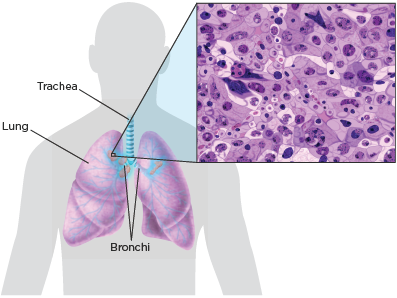
\includegraphics[width=\textwidth]{Images/chapter_1/large_cell.png}
%    \caption{Large cell carcinoma.}
%    \label{fig:large_cell}
%    \end{subfigure}
%    \caption{Location and histology of the NSCLC \cite{}.}
%    \label{fig:NSCLC_types}
%\end{figure}

Classifying NSCLC tumors into histological subtypes was the first step towards a better distinction of the molecular, phenotypical, and prognostic features of NSCLC and became the first approach to develop personalized treatment strategies based on the tumor characteristics. However, the development of molecular biology techniques applied to the study of cancer revealed the complexity of genomic and epigenetic differences between these histological subtypes, unraveling the existence of potent oncogenic drivers in lung adenocarcinomas and giving rise to the era of targeted therapies for this disease \cite{Mol_bio}.

\subsection{Molecular Classification of Lung Adenocarcinomas}

Lung adenocarcinomas are classified according to the presence of well-identified and characterized molecular alterations that drive cancer initiation and progression. This genomic classification relies on the detection of copy number variations due to deletions, duplications, or amplification and gene fusions driven by insertions, inversions, and translocations in key genes. Ultimately, these alterations translate at the functional level into the activation of oncogenes and the inactivation of tumor suppressor genes \cite{Mol_markers, Gene_express}, which play a crucial role in signal transduction, cellular proliferation, differentiation, and other regulatory mechanisms (\autoref{fig:Pathway}).

\begin{figure}[t]
    \centering
    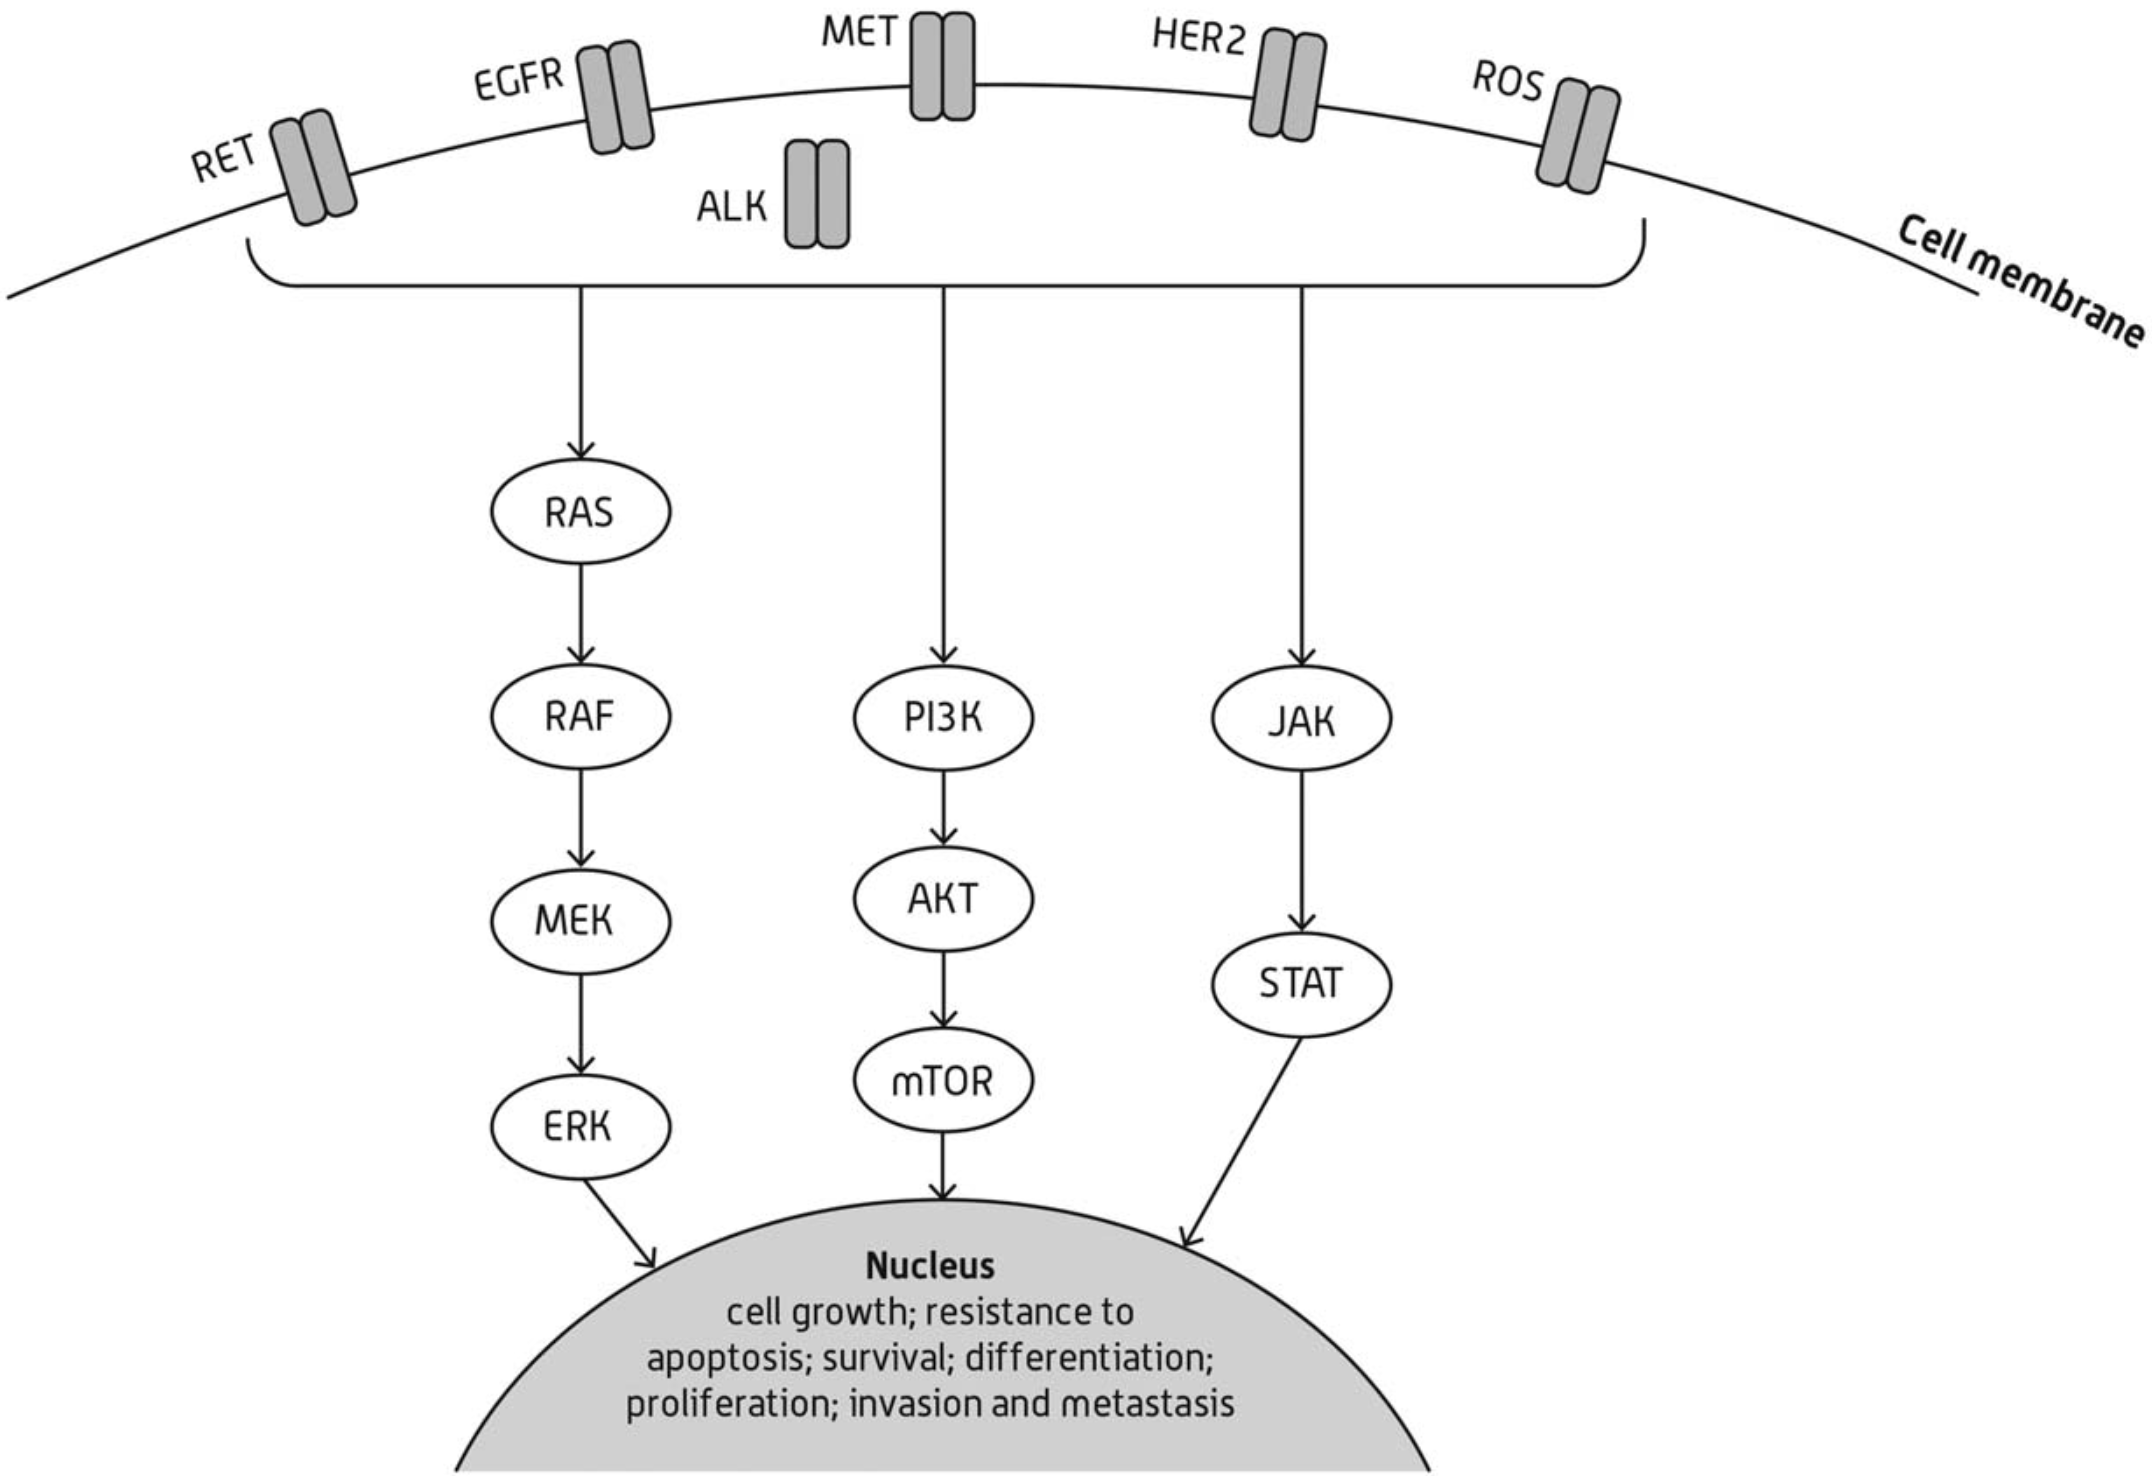
\includegraphics[width=0.9\textwidth]{Images/chapter_1/molecular_pathway.png}
    \caption{Molecular pathways of non-small cell lung cancer. AKT, protein kinase B; ALK, anaplastic lymphoma kinase; EGFR, epidermal growth factor receptor; ERK, extracellular signal-regulated kinase; HER2, human epidermal growth factor receptor 2; JAK, janus kinase; MEK, mitogen-activated protein kinase kinase; MET, mesenchymal-to-epithelial transition; mTOR, mammalian target of rapamycin; PI3K, phosphoinositide 3-kinase; RAF, rapidly accelerated fibrosarcoma; RAS, rat sarcoma; RET, rearranged during transfection; ROS, reactive oxygen species; STAT, signal transducer and activator of transcription proteins. Modified image from \cite{NSCLC_drivers}.}
    \label{fig:Pathway}
\end{figure}

The most relevant driver mutations leading to the classification of genomic subtypes of lung adenocarcinoma are KRAS, EGFR, ALK, ROS1, BRAF, RET, NTRK1, NRG1, HER2 (also named ERBB2), and MET. The prevalence of each of these mutations, as well as the notable differences between the oncogenic paradigm of the early and more advanced stages of this disease, are reflected in \autoref{fig:Drivers}. It must also be taken into consideration that this distribution is not uniform worldwide and that there are significant changes depending on the different geographical areas \cite{Mol_bio}.

\begin{figure}[ht]
    \centering
    \begin{subfigure}{0.49\textwidth}
        \centering
        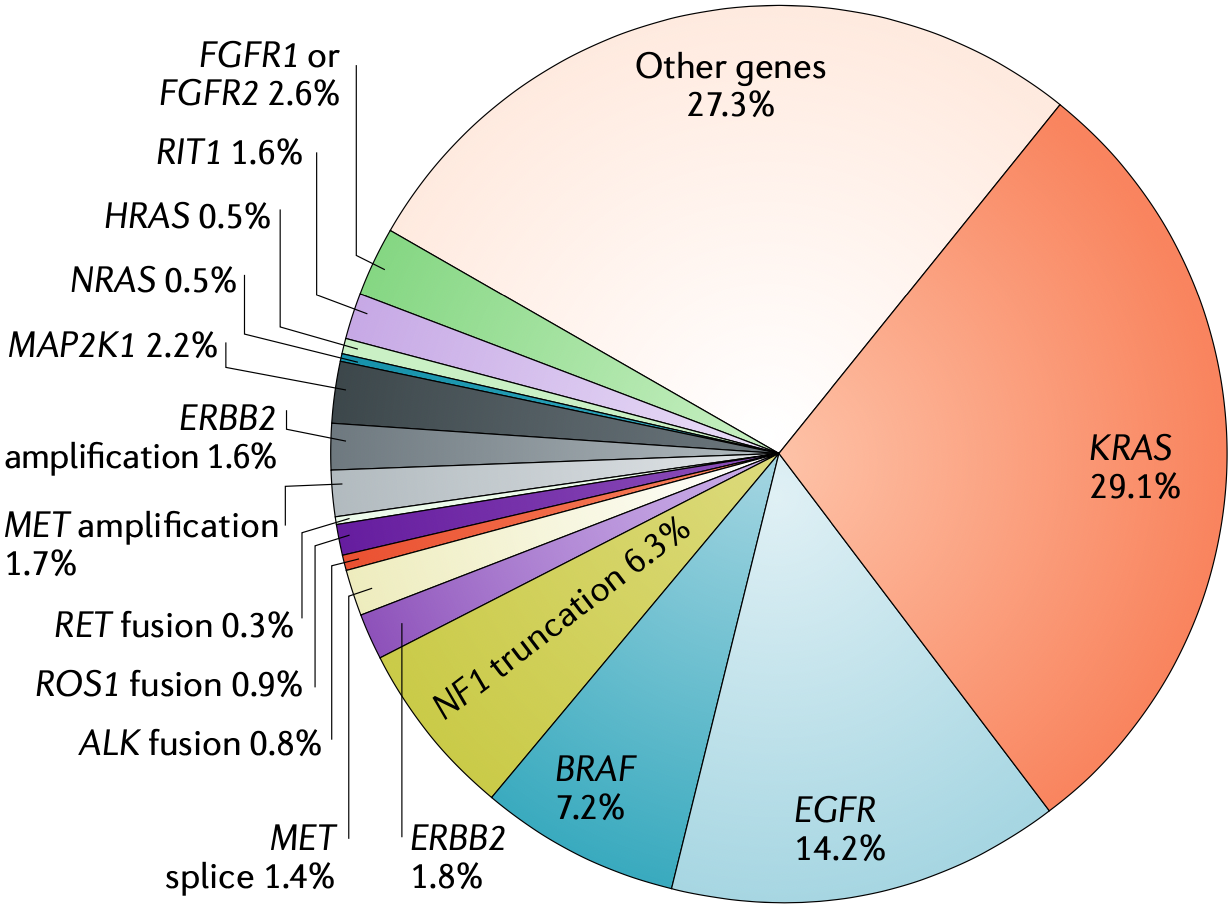
\includegraphics[width=\textwidth]{Images/chapter_1/drivers_early.png}
        \caption{Early-stage adenocarcinoma.}
        \label{fig:Drivers_early}
    \end{subfigure}
    \hfill
    \begin{subfigure}{0.49\textwidth}
        \centering
        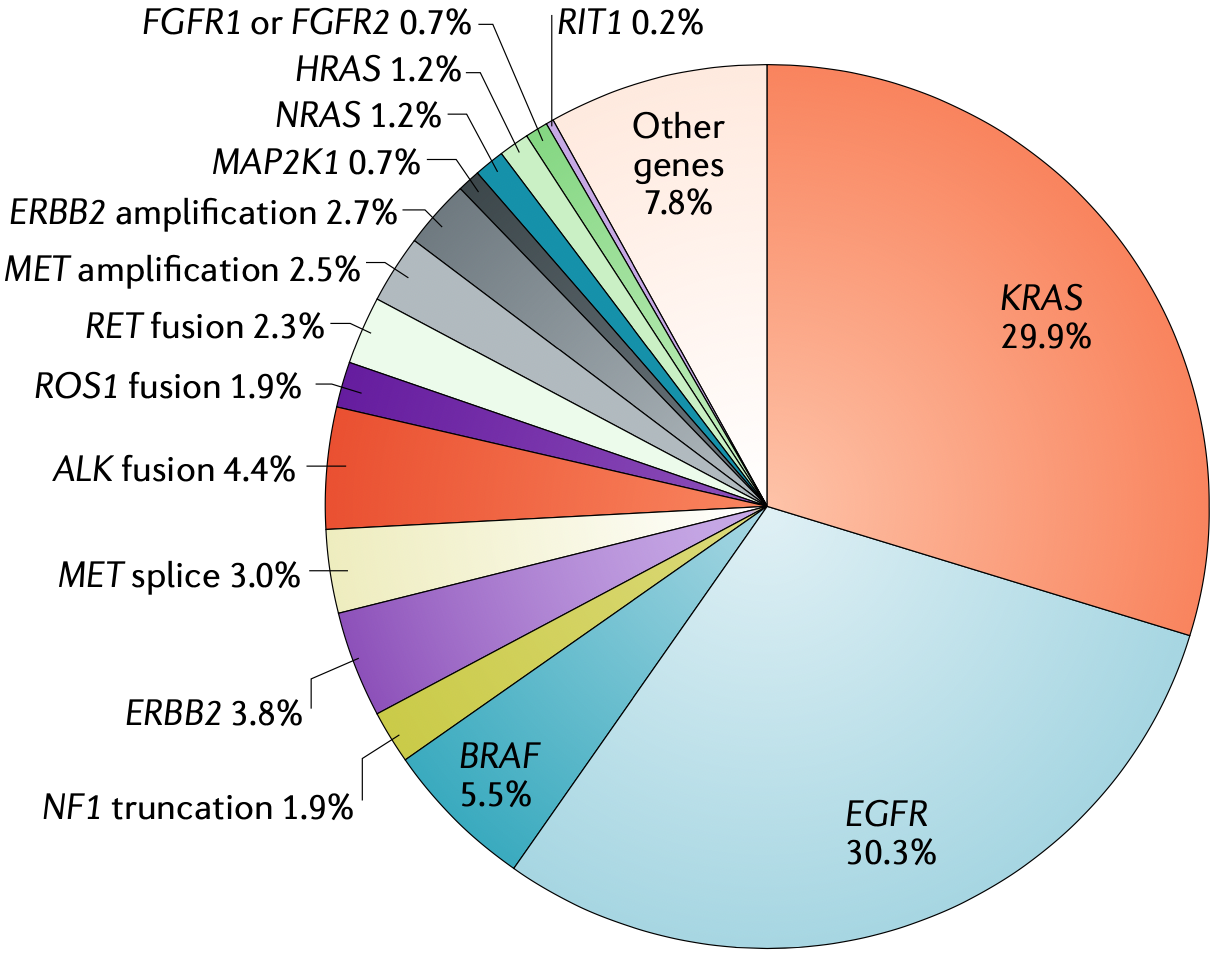
\includegraphics[width=\textwidth]{Images/chapter_1/drivers_metastasis.png}
        \caption{Metastatic-stage adenocarcinoma.}
        \label{fig:Drivers_metastasis}
    \end{subfigure}
    \caption{Oncogenic driver paradigm of lung adenocarcinoma molecular classification. Modified images from \cite{NSCLC_alterations}.}
    \label{fig:Drivers}
\end{figure}

Up to 50\% of all lung cancers patients harbor a genetic alteration and 20\% have a targetable mutation \cite{NSCLC_profiling}. Therefore, whenever feasible, patients with advanced NSCLC should have tumor assessed for the presence of a driver alteration \cite{Mol_guideline_1}. However, guidelines from the College of American Pathologists (CAP), the International Association for the Study of Lung Cancer (IASLC) and the Association of Molecular Pathologists (AMP) recommend analysis of either the primary tumor or of metastasis for EGFR and ALK, which are mutually exclusive, for all patients whose tumor contains an element of adenocarcinoma and regardless of the clinical characteristics of the subjects \cite{Mol_guideline_1, Mol_guideline_2}. The reason is that certain genetic changes, such as EGFR mutations or ALK translocations are strongly associated with a positive targeted therapeutic response. For other prevalent mutations such as KRAS, for which preclinical studies have nominated targeted approaches, the clinical utility has yet to be established \cite{KRAS}.

Regarding co-occurring genomic alterations, they have emerged as core  determinants of the molecular and clinical heterogeneity in different NSCLC subgroups, including those driven by EGFR mutations and ALK translocations. Specifically, these subgroups are dominated by co-occurring TP53 alterations, PIK3CA mutations, and FGFR1 amplifications \cite{NSCLC_alterations}.

\subsubsection{Epidermal Growth Factor Receptor (EGFR)}

Driver mutations in the EGFR gene (chromosome 7) can be found in 10–20\% of the Caucasian population diagnosed with NSCLC, but are more prevalent in Asians (35–45\%) \cite{AD_drivers, AD_asian}. Patients who are women, nonsmokers, and diagnosed with a pulmonary adenocarcinoma are more likely to harbor an EGFR mutation, but it can also be found in subjects without these characteristics \cite{Mol_bio}.

EGFR is one of the four members of the family of membrane receptors with tyrosine kinase activity known as ERBB. Activation of this receptor leads to both increased cell proliferation and slowed apoptosis by stimulating oncogenic pathways such as MAPK\slash ERK, also known as RAS\slash RAF\slash MEK\slash ERK, and PI3K\slash AKT\slash mTOR (\autoref{fig:Pathway}).

This type of EGFR activating mutations in NSCLC, and discovered in 2004, is located in exons 18–21, which encode part of the tyrosine kinase domain. However, 90\% of these alterations are exon 19 in-frame deletions of amino acids 747–750 (45\%) and exon 21 mutations resulting in L858R substitutions (40–45\%) \cite{EGFR}. The remaining 10\% of mutations involve exons 18 and 20.

\subsubsection{Anaplastic Lymphoma Kinase (ALK)} \label{sec:ALK}

ALK rearrangements are oncogenic drivers that occur in 3–7\% of patients with NSCLC and are more common among younger patients with a light smoking history, adenocarcinoma histology, and absence of EGFR and KRAS mutations \cite{NSCLC_drivers, AD_drivers}.

ALK promotes the downstream activation of proliferative and anti-apoptotic signals via intracellular pathways \cite{ALK_fusions, EML4_ALK}, including Ras\slash ERK, PI3K\slash AKT, and JAK\slash STAT (\autoref{fig:Pathway}), which eventually culminate in oncogenesis.

In ALK-activated NSCLC, the predominant molecular event leading to ALK activation is the juxtaposition of the N-terminal portion of the protein encoded by the echinoderm microtubule-associated protein-like 4 (EML4) gene with the intracellular domain of the ALK tyrosine kinase \cite{ALK_identification}. This somatic rearrangement was first described as a molecular driver in a small cohort of Japanese NSCLC patients in 2007 \cite{ALK_identification}. Ever since 15 distinct variants of EML4-ALK have been identified with some of them being expressed as multiple isoforms. Variants 1, 2 and 3a\slash b are the most common  (\autoref{fig:EML4-ALK_frequency}), accounting for around 90\% of all cases \cite{EML4_ALK_variants}, and as described previously, all of them include the kinase domain of ALK, encoded by exons 20–29, but differ in size based on the EML4 breakage point  (\autoref{fig:EML4-ALK_variants}).

\begin{figure}[t]
    \centering
    \begin{subfigure}{0.64\textwidth}
        \centering
        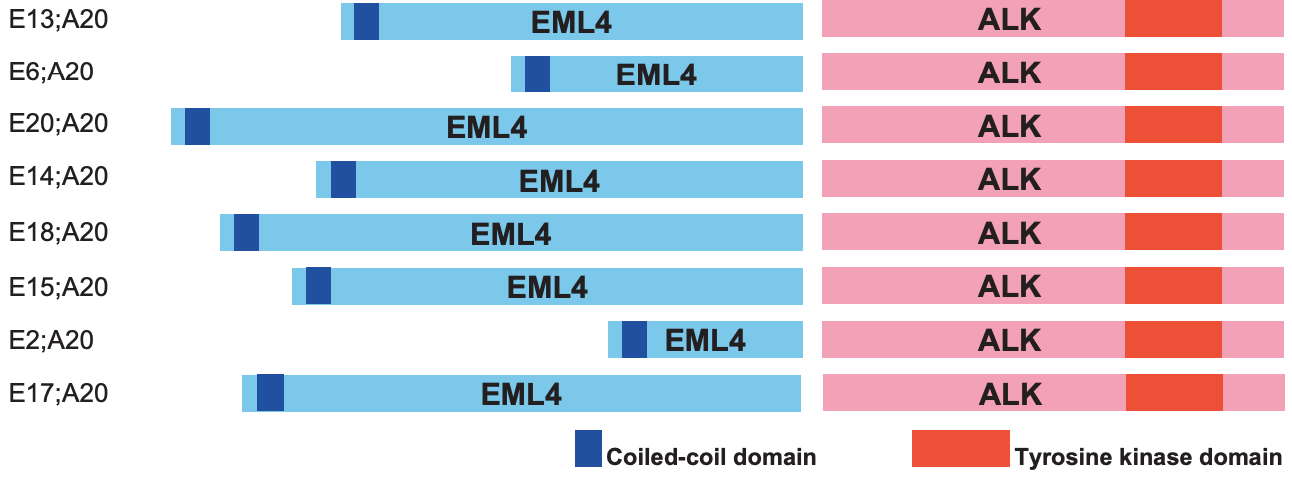
\includegraphics[width=\textwidth]{Images/chapter_1/variants_EML4-ALK.png}
        \caption{EML4-ALK main variants.}
        \label{fig:EML4-ALK_variants}
    \end{subfigure}
    \hfill
    \begin{subfigure}{0.34\textwidth}
        \centering
        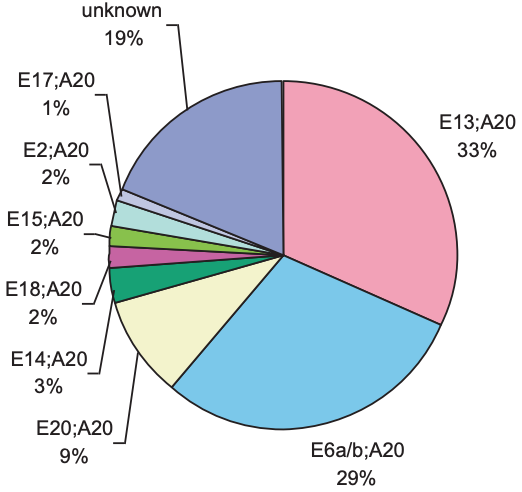
\includegraphics[width=\textwidth]{Images/chapter_1/frequency_variants_EML4-ALK.png}
        \caption{Frequency of different EML4-ALK variants.}
        \label{fig:EML4-ALK_frequency}
    \end{subfigure}
    \caption{Different variants of EML4-ALK. The most common variants are E13;A20 (variant 1), E20;A20 (variant 2) and E6a\slash b;A20 (variant 3). The nomenclature refers to the exon in EML4 translocated to the exon in ALK. Modified images from \cite{EML4_ALK_biology}.}
    \label{fig:EML4-ALK}
\end{figure}

\subsection{International Staging System: the TNM Classification}

Cancer staging is a critical step in the diagnostic process and its objectives are multiple \cite{TNM}, including:
\begin{itemize}
    \item Aid treatment planning.
    \item Provide an indication of prognosis.
    \item Assist in the evaluation of treatment results.
    \item Facilitate the exchange of information between treatment centers.
    \item Contribute to continuing investigations of human malignancies.
\end{itemize}

The fundamental structure of stage classification is the TNM system, which since its introduction in the 1970s has undergone significant revisions with the latest, 8th edition, being effective internationally from 2018 \cite{TNM_8th}. It describes the anatomical extent of the disease and, using alphanumeric codes, NSCLC is typically given a clinical stage based on the results of a physical exam, biopsy, and imaging tests.

\subsubsection{Tumor Staging (T)}

The T stage is determined by the size of the primary tumor in the long axis measured in multiplanar reconstruction and its involvement with the adjacent structures (\autoref{tab:T_descriptors}).

\begin{table}[ht]
\centering
\resizebox{0.95\textwidth}{!}{
\renewcommand{\arraystretch}{1.5}
\begin{tabular}{lcp{18cm}}
\rowcolor[HTML]{EFEFEF} 
    \multicolumn{2}{l}{\cellcolor[HTML]{EFEFEF}\textbf{Tx}} & Primary tumor cannot be assessed or tumor is proven by the presence of malignant cells in sputum or bronchial washings but not visualized by imaging or bronchoscopy \\
\rowcolor[HTML]{FFFFFF} 
    \multicolumn{2}{l}{\cellcolor[HTML]{FFFFFF}\textbf{T0}} & No evidence of primary tumor \\
\rowcolor[HTML]{EFEFEF} 
    \multicolumn{2}{l}{\cellcolor[HTML]{EFEFEF}\textbf{Tis}} & Carcinoma in situ \\
\rowcolor[HTML]{FFFFFF} 
    \multicolumn{2}{l}{\cellcolor[HTML]{FFFFFF}\textbf{T1}} & Tumor $\le 3$ $cm$ in greatest dimension, surrounded by lung or visceral pleura, without bronchoscopic evidence of invasion more proximal than the lobar bronchus (i.e., not in the main bronchus) \\
        \rowcolor[HTML]{FFFFFF} & \textbf{T1mi} & Minimally invasive adenocarcinoma: solitary adenocarcinoma, $\le 3$ $cm$ with a predominantly lepidic pattern and $\le 5$ mm invasion in greatest dimension \\
        \rowcolor[HTML]{FFFFFF} & \textbf{T1a} & Tumor $\le 1$ $cm$ in greatest dimension \\
        \rowcolor[HTML]{FFFFFF} & \textbf{T1b} & Tumor $> 1$ $cm$ but $\le 2$ $cm$ in greatest dimension \\
        \rowcolor[HTML]{FFFFFF} & \textbf{T1c} & Tumor $> 2$ $cm$ but $\le 3$ $cm$ in greatest dimension \\
\rowcolor[HTML]{EFEFEF} 
    \multicolumn{2}{l}{\cellcolor[HTML]{EFEFEF}\textbf{T2}} & Tumor $> 3$ $cm$ but $\le 5$ $cm$ or having any of the following features: \newline
    - Involves main bronchus regardless of distance from the carina, but without the involvement of the carina \newline
    - Invades visceral pleura \newline
    - Associated with atelectasis or obstructive pneumonitis that extends to the hilar region, involving part or all of the lung \\
        \rowcolor[HTML]{EFEFEF} & \textbf{T2a} & Tumor $> 3$ $cm$ but $\le 4$ $cm$ in greatest dimension \\
        \rowcolor[HTML]{EFEFEF} & \textbf{T2b} & Tumor $> 4$ $cm$ but $\le 5$ $cm$ in greatest dimension \\
\rowcolor[HTML]{FFFFFF} 
    \multicolumn{2}{l}{\cellcolor[HTML]{FFFFFF}\textbf{T3}} & Tumor $> 5$ $cm$ but $\le 7$ $cm$ in greatest dimension or associated with separate tumor nodule(s) in the same lobe as the primary tumor or directly invades any of the following structures: chest wall (including the parietal pleura and superior sulcus tumors), phrenic nerve and parietal pericardium \\
\rowcolor[HTML]{EFEFEF}
    \multicolumn{2}{l}{\cellcolor[HTML]{EFEFEF}\textbf{T4}} & Tumor $> 7$ $cm$ in greatest dimension or associated with separate tumor nodule(s) in a different ipsilateral lobe than that of the primary tumor or invades any of the following structures: diaphragm, mediastinum, heart, great vessels, trachea, recurrent laryngeal nerve, esophagus, vertebral body and carina
\end{tabular}}
\caption{T-descriptors of the TNM classification for lung cancer \cite{TNM_proposal}.}
\label{tab:T_descriptors}
\end{table}

\subsubsection{Nodal Staging (N)}

The nodal staging assesses tumor burden in the regional hilar and mediastinal nodes (\autoref{tab:N_descriptors}).

\begin{table}[ht]
\centering
\resizebox{0.95\textwidth}{!}{
\renewcommand{\arraystretch}{1.5}
\begin{tabular}{lcp{18cm}}
\rowcolor[HTML]{EFEFEF} 
    \multicolumn{2}{l}{\cellcolor[HTML]{EFEFEF}\textbf{Nx}} & Regional lymph nodes cannot be assessed \\
\rowcolor[HTML]{FFFFFF} 
    \multicolumn{2}{l}{\cellcolor[HTML]{FFFFFF}\textbf{N0}} & No regional node metastasis \\
\rowcolor[HTML]{EFEFEF} 
    \multicolumn{2}{l}{\cellcolor[HTML]{EFEFEF}\textbf{N1}} & Metastasis in ipsilateral peribronchial and\slash or ipsilateral hilar lymph nodes and intrapulmonary nodes, including involvement by direct extension \\
\rowcolor[HTML]{FFFFFF} 
    \multicolumn{2}{l}{\cellcolor[HTML]{FFFFFF}\textbf{N2}} & Metastasis in ipsilateral mediastinal and\slash or subcarinal lymph node(s) \\
\rowcolor[HTML]{EFEFEF}
    \multicolumn{2}{l}{\cellcolor[HTML]{EFEFEF}\textbf{N3}} & Metastasis in the contralateral mediastinal, contralateral hilar, ipsilateral or contralateral scalene or supraclavicular lymph node(s)
\end{tabular}}
\caption{N-descriptors of the TNM classification for lung cancer \cite{TNM_proposal}.}
\label{tab:N_descriptors}
\end{table}

\subsubsection{Metastasis Staging (M)}

M staging is defined by the presence of metastasis beyond the regional lymph nodes (\autoref{tab:M_descriptors}).

\begin{table}[ht]
\centering
\resizebox{0.95\textwidth}{!}{
\renewcommand{\arraystretch}{1.5}
\begin{tabular}{lcp{18cm}}
\rowcolor[HTML]{EFEFEF} 
    \multicolumn{2}{l}{\cellcolor[HTML]{EFEFEF}\textbf{M0}} & No distant metastasis \\
\rowcolor[HTML]{FFFFFF} 
    \multicolumn{2}{l}{\cellcolor[HTML]{FFFFFF}\textbf{M1}} & Distant metastasis \\
        \rowcolor[HTML]{FFFFFF} & \textbf{M1a} & Separate tumor nodule(s) in a contralateral lobe tumor; tumor with pleural or pericardial nodules or malignant pleural or pericardial effusion \\
        \rowcolor[HTML]{FFFFFF} & \textbf{M1b} & Single extrathoracic metastasis in a single organ and involvement of a single nonregional lymph node \\
        \rowcolor[HTML]{FFFFFF} & \textbf{M1c} & Multiple extrathoracic metastases in a single or multiple organs
\end{tabular}}
\caption{M-descriptors of the TNM classification for lung cancer \cite{TNM_proposal}.}
\label{tab:M_descriptors}
\end{table}

\subsubsection{Stage Grouping}

All possible combinations of the T, N, and M categories are used to create TNM subsets (\autoref{tab:TNM_staging}), which are then combined into stage groupings that share similar prognoses, ranging from one to four (I through IV).

\begin{table}[ht]
\centering
\resizebox{0.40\textwidth}{!}{
\renewcommand{\arraystretch}{1.1}
\begin{tabular}{lccc}
\rowcolor[HTML]{EFEFEF} \textbf{Occult carcinoma} & TX & N0 & M0 \\
\rowcolor[HTML]{FFFFFF} \textbf{Stage 0} & Tis & N0 & M0 \\
\rowcolor[HTML]{EFEFEF} \cellcolor[HTML]{EFEFEF} & T1mi & N0 & M0 \\
\rowcolor[HTML]{EFEFEF} \multirow{-2}{*}{\cellcolor[HTML]{EFEFEF}\textbf{Stage IA1}}  & T1a & N0 & M0 \\
\rowcolor[HTML]{FFFFFF} \textbf{Stage IA2} & T1b & N0 & M0 \\
\rowcolor[HTML]{EFEFEF} \textbf{Stage IA3} & T1c & N0 & M0 \\
\rowcolor[HTML]{FFFFFF} \textbf{Stage IB} & T2a & N0 & M0 \\
\rowcolor[HTML]{EFEFEF} \textbf{Stage IIA} & T2b & N0 & M0 \\
\rowcolor[HTML]{FFFFFF} \cellcolor[HTML]{FFFFFF} & T1a-c & N1 & M0 \\
\rowcolor[HTML]{FFFFFF} \cellcolor[HTML]{FFFFFF} & T2a & N1 & M0 \\
\rowcolor[HTML]{FFFFFF} \cellcolor[HTML]{FFFFFF} & T2b & N1 & M0 \\
\rowcolor[HTML]{FFFFFF} \multirow{-4}{*}{\cellcolor[HTML]{FFFFFF}\textbf{Stage IIB}} & T3 & N0 & M0 \\
\rowcolor[HTML]{EFEFEF} \cellcolor[HTML]{EFEFEF} & T1a-c & N2 & M0 \\
\rowcolor[HTML]{EFEFEF} \cellcolor[HTML]{EFEFEF} & T2a-b & N2 & M0 \\
\rowcolor[HTML]{EFEFEF} \cellcolor[HTML]{EFEFEF} & T3 & N1 & M0 \\
\rowcolor[HTML]{EFEFEF} \cellcolor[HTML]{EFEFEF} & T4 & N0 & M0 \\
\rowcolor[HTML]{EFEFEF} \multirow{-5}{*}{\cellcolor[HTML]{EFEFEF}\textbf{Stage IIIA}} & T4 & N1 & M0 \\
\rowcolor[HTML]{FFFFFF} \cellcolor[HTML]{FFFFFF} & T1a-c & N3 & M0 \\
\rowcolor[HTML]{FFFFFF} \cellcolor[HTML]{FFFFFF} & T2-ab & N3 & M0 \\
\rowcolor[HTML]{FFFFFF} \cellcolor[HTML]{FFFFFF} & T3 & N2 & M0 \\
\rowcolor[HTML]{FFFFFF} \multirow{-4}{*}{\cellcolor[HTML]{FFFFFF}\textbf{Stage IIIB}} & T4 & N2 & M0 \\
\rowcolor[HTML]{EFEFEF} \cellcolor[HTML]{EFEFEF} & T3 & N3 & M0 \\
\rowcolor[HTML]{EFEFEF} \multirow{-2}{*}{\cellcolor[HTML]{EFEFEF}\textbf{Stage IIIC}} & T4 & N3 & M0 \\
\rowcolor[HTML]{FFFFFF} \cellcolor[HTML]{FFFFFF} & Any T & Any N & M1a \\
\rowcolor[HTML]{FFFFFF} \multirow{-2}{*}{\cellcolor[HTML]{FFFFFF}\textbf{Stage IVA}} & Any T & Any N & M1b \\
\rowcolor[HTML]{EFEFEF} \textbf{Stage IVB} & Any T & Any N & M1c
\end{tabular}}
\caption{Lung cancer stage grouping \cite{TNM_proposal}.}
\label{tab:TNM_staging}
\end{table}

\subsection{Current Treatment Options}

The treatment of pulmonary adenocarcinoma depends on several factors including stage, resectability, performance status, histology, and genomic alterations acquired by the individual tumor \cite{NSCLC}. As in most types of cancer, treatment approaches can be divided into 5 categories: surgery, chemotherapy, radiotherapy, immunotherapy, and targeted therapy.

\subsubsection{Surgical Resection}

Surgery is the most effective therapy for stages I to II and selected cases of stage IIIA NSCLC \cite{NSCLC_therapies}. To determine if the tumor is resectable, imaging studies and biopsies are completed as well as an evaluation of the patient to verify if the surgery will be tolerable. In this procedure, surgeons can perform a lobectomy if the tumor is located only in one lobe, or a pneumonectomy if it affects more than one lobe or the main bronchus. This latter intervention carries significant operative mortality and long-term morbidity, although outcomes are currently improving for resectable early-stage lung cancer owing to advances in minimally invasive thoracic surgery technologies such as video-assisted thoracoscopic surgery (VATS) \cite{VATS}. However, despite the progress being made in this field, a high percentage of tumors will recur, with 5-year overall survival ranging from 83\% for stage IA to 36\% for stage IIIA disease \cite{TNM_proposal}.

On the other hand, some patients who have undergone resection surgery may benefit from adjuvant therapy. It may include radiation, chemotherapy, and targeted therapy and is associated with improved survival in patients with resected stage II and IIIA NSCLC \cite{Adjuvant}.

\subsubsection{Chemotherapy}

Chemotherapy has been the mainstay of treatment in patients with advanced (stage IV) and unresectable lung tumors for approximately 3 decades and it is currently given with palliative intent. The first-line therapy is platinum-based doublet chemotherapy, combining cisplatin or carboplatin with another cytotoxic agent and the regimens might be influenced by the patients' histology, age, comorbidity, performance status, response and molecular genetic features of cancer \cite{NSCLC_therapies}.

Approximately 40\% of newly diagnosed lung cancer patients are stage IV and their median overall survival (OS) is $4.5$ months when no chemotherapy is given \cite{TNM}. However, the 1-year OS improves from 10–20\% up to 30–50\%  with chemotherapy, reducing disease-related adverse events \cite{EGFR_mutations}.

\subsubsection{Radiotherapy}

Radiation therapy delivers high-energy ionizing radiation to destroy cancer cells by damaging their DNA. Therefore, it can help control or eliminate tumors at specific sites in the body. In the treatment of stage I and stage II NSCLC, this treatment alone is considered only when the tumor is unresectable, being associated with a 3-year cancer-specific survival rate approaching 55\% in early-stage lung cancer \cite{Radio}. However, it also can be part of palliative care to improve quality of life in NSCLC patients who do not respond to surgery or chemotherapy or as adjuvant therapy for patients who have undergone a resection surgery to reduce the risk of lung cancer relapse.

\subsubsection{Immunotherapy}

Immunotherapy is a breakthrough treatment in oncology that uses the patients' immune system to fight off cancer. Since some tumor cells share characteristics with healthy cells, the goal is to stimulate the host's immune system so that it can target cancer cells, stopping or slowing their growth and preventing their spread to other parts of the body. 

Therapeutic approaches that modulate the immune system in patients with lung cancer have traditionally concentrated on vaccines and have generally been ineffective. However, most recent approaches focused on a series of ligands and receptors that inhibit or stimulate the immunological synapse have been approved for the treatment of patients with metastatic NSCLC and have been shown in several randomized trials to lead to better outcomes compared to standard chemotherapy \cite{Immuno}. Specifically, these new strategies are targeting immune checkpoint pathways, which include the blockade of the inhibitory receptors cytotoxic T-lymphocyte-associated antigen 4 (CTLA-4) and programmed cell death 1 (PD-1) and its ligand, PD-L1.

\subsubsection{Targeted Therapy} \label{sec:Targeted}

The identification of targetable gene alterations has dramatically transformed the management of malignant tumors, allowing individualized therapy, and leading to remarkable responses in selected patients treated with matched tyrosine kinase inhibitors (TKIs). Therefore, it is a successful strategy and results in improved OS of patients with a driver mutation as compared to patients with a driver mutation that do not receive targeted therapy \cite{Targeted_drugs}. In addition, the toxicity profile, in this case, is milder compared to conventional chemotherapy.

Targeted therapies using EGFR TKIs against tumors with EGFR mutations and ALK TKIs against tumors with ALK fusions thus has become an increasingly standard treatment in clinical settings. Currently, almost all guidelines recommend the use of EGFR TKIs, such as Gefitinib (Iressa\textsuperscript\textregistered{}), Erlotinib (Tarceva\textsuperscript\textregistered{}) or Afatinib (Gilotrif\textsuperscript\textregistered{}), and ALK TKIs, such as Crizotinib (Xalkori\textsuperscript\textregistered{}) and Alectinib (Alecensa\textsuperscript\textregistered{}), as first-line treatments \cite{Mol_bio, ALK_fusions, NSCLC_therapies}. Through genomic testing, other molecular changes have been found including gene rearrangements of ROS1 and RET, amplification of MET, and activating mutations in BRAF, HER2, and KRAS genes (\autoref{tab:Alterations}). However, most lung adenocarcinomas either lack an identifiable driver oncogene or harbor mutations that are more responsive to chemotherapy due to the lack of truly effective drugs \cite{Mol_profiling}.

\begin{table}[ht]
\centering
\resizebox{\textwidth}{!}{
\renewcommand{\arraystretch}{1.5}
\begin{tabular}{clcl}
\rowcolor[HTML]{C0C0C0} 
\textbf{Gene} & \multicolumn{1}{c}{\cellcolor[HTML]{C0C0C0}\textbf{Most Common Alteration}} & \textbf{Prevalence} & \multicolumn{1}{c}{\cellcolor[HTML]{C0C0C0}\textbf{Treatment}} \\
% EGFR
\textbf{EGFR} & \begin{tabular}[c]{@{}l@{}}Exon 19 deletion \\ and exon 21 activating mutation\end{tabular} & 15–35\% & \begin{tabular}[c]{@{}l@{}}Erlotinib (Tarceva\textsuperscript\textregistered{}), Afatinib (Gilotrif\textsuperscript\textregistered{}), Gefitinib (Iressa\textsuperscript\textregistered{}), \\ Osimertinib (Tagrisso\textsuperscript\textregistered{}), Dacomitinib (Vizimpro\textsuperscript\textregistered{})\end{tabular} \\
% ALK
\rowcolor[HTML]{EFEFEF} \textbf{ALK}  & \begin{tabular}[c]{@{}l@{}}Fusion of partner gene\\ with exon 20 of ALK\end{tabular} & 3–7\% & \begin{tabular}[c]{@{}l@{}}Crizotinib (Xalkori\textsuperscript\textregistered{}), Ceritinib (Zykadia\textsuperscript\textregistered{}), Alectinib (Alecensa\textsuperscript\textregistered{}), \\ Brigatinib (Alunbrig\textsuperscript\textregistered{}), Lorlatinib (Lorbrena\textsuperscript\textregistered{})\end{tabular} \\
% KRAS
\textbf{KRAS} & Codon 12 mutation & 25–30\% & AMG 510, MRTX849 \\ \rowcolor[HTML]{EFEFEF} \textbf{BRAF} & V600E mutation & 3–5\% & \begin{tabular}[c]{@{}l@{}}Dabrafenib (Tafinlar\textsuperscript\textregistered{}) + Trametinib (Mekinist\textsuperscript\textregistered{}), \\ Vemurafenib (Zelboraf\textsuperscript\textregistered{})\end{tabular} \\
% ROS1
\textbf{ROS1} & Translocation & $\sim 2$\% & \begin{tabular}[c]{@{}l@{}}Crizotinib (Xalkori\textsuperscript\textregistered{}), Ceritinib (Zykadia\textsuperscript\textregistered{}), Lorlatinib (Lorbrena\textsuperscript\textregistered{}), \\ Entrectinib (Rozlytrek\textsuperscript\textregistered{})\end{tabular} \\
% RET
\rowcolor[HTML]{EFEFEF} \textbf{RET} & Translocation & $\sim 2$\% & \begin{tabular}[c]{@{}l@{}}Multitarget TKIs such as Cabozantinib (Cabometyx\textsuperscript\textregistered{}), Vandetanib \\ (Caprelsa\textsuperscript\textregistered{}) and Alectinib (Alecensa\textsuperscript\textregistered{}), and selective  RET inhibitors \\ such as LOXO-292 (Selpercatinib\textsuperscript\textregistered{}) and BLU667 (Pralsetinib\textsuperscript\textregistered{})\end{tabular} \\
% MET
\textbf{MET} & \begin{tabular}[c]{@{}l@{}}Amplification \\ and exon 14 skipping mutation\end{tabular} & $\sim 3$\% & Crizotinib (Xalkori\textsuperscript\textregistered{}), Glesatinib, Capmatinib \\
% HER2
\rowcolor[HTML]{EFEFEF} \textbf{HER2} & Activating exon 20 in-frame insertion & 2–3\% & Poziotinib, Afatinib (Gilotrif\textsuperscript\textregistered{}), Trastuzumab-emtansine (Kadcyla\textsuperscript\textregistered{})
\end{tabular}}
\caption{Overview of driver genetic alterations potentially amenable to targeted treatment \cite{EGFR_mutations, EML4_ALK, KRAS_drugs, BRAF, ROS1, RET, MET, HER2, NSCLC_therapies}. The most common alterations as well as their prevalence are shown along with the main treatments, including both those approved and marketed and those that are undergoing clinical trials.}
\label{tab:Alterations}
\end{table}

The presence of genetic alterations, which leads to the use of targeted agents as first-line therapy, is associated with improved progression-free survival (PFS), 10 versus 7.1 months, and OS, 16.5 versus 11.8 months, according to a nationwide French study \cite{NSCLC_profiling}. Similarly, in the United States, the Lung Cancer Mutation Consortium conducted a study reflecting that the median survival was 3.5 years for patients with an oncogenic driver and genotype-directed therapy, compared to 2.4 years for subjects with any oncogenic drivers and therefore not eligible for targeted therapy \cite{Targeted_drugs}.

However, despite the initial efficacy of these inhibitors, patients eventually develop acquired drug resistance within 1 to 2 years from the start of TKI treatment, regardless of the line of therapy \cite{TKI_resistance}. In this way, efforts are currently focusing on identifying new therapeutic biomarkers, generating next-generation drugs to overcome drug resistance, and developing methods to diagnose driver gene mutations using less invasive biopsy techniques, such as liquid biopsy.

In this thesis, only the identification of ALK rearrangements in NSCLC patients with adenocarcinoma histology will be addressed.

\subsubsection{Angiogenesis Inhibitors}

Angiogenesis, which is the formation of new blood vessels, is essential in the process of primary tumor growth and is, therefore, a critical step toward local and systemic spread. The main signaling pathways that have been identified to regulate tumor angiogenesis include vascular endothelial growth factor (VEGF), platelet-derived growth factor (PDGF), and fibroblast growth factor (FGF). However, targeting tumor angiogenesis is currently being approached through two primary methods, monoclonal antibodies that block the VEGF-vascular endothelial growth factor receptor (VEGFR) binding or small-molecule TKI that inhibit the VEGF pathway \cite{Angiogenesis}.

\section{ALK-Positive Non-Small Cell Lung Cancer}

As mentioned in \autoref{sec:ALK}, EML4-ALK variants are the most common ALK rearrangement seen in NSCLC patients.

Anaplastic lymphoma kinase is a 1,620 amino acid transmembrane protein and is a member of the insulin receptor tyrosine kinases. It was originally identified in 1994 in anaplastic large-cell lymphoma (ALCL) as a fusion to a part of the nucleophosmin (NPM) protein. On the other hand, echinoderm microtubule-associated protein-like 4 (EML4) is a cytoplasmic protein essential for the formation of microtubules and microtubule-binding protein.

EML4 and ALK are closely located genes situated only 12.7 megabases apart on the short arm of chromosome 2, 2p21 and 2p23, respectively. Inversion of this part of the short arm of chromosome 2 [Inv(2)(p21p23)], that juxtaposed the 5' end of the EML4 gene with the 3' end of the ALK gene, creates a fusion between these two genes by joining exons 1–13 of EML4 to exons 20–29 of ALK (\autoref{fig:EML4-ALK_variants}).

As described in \autoref{sec:ALK} and \autoref{sec:Targeted}, since its discovery in lung adenocarcinomas in 2007 and the subsequent identification of at least 15 different variants through reverse transcription polymerase chain reaction (RT-PCR) or next generation sequencing (NGS) \cite{EML4_ALK_variants}, there has been a revolution in molecular-targeted therapy that has transformed the outlook for NSCLC patients.

\subsection{Current Therapeutic Agents: Targeted ALK Inhibitors}

Advanced NSCLC associated with the ALK fusion oncogene is highly sensitive to ALK tyrosine kinase inhibitors (TKIs), which represent a newer group of medications that prevents intracellular signaling from the ALK alteration, leading to decreased cellular proliferation. However, due to the acquisition of secondary mutations and the activation of alternative pathways, it is common for patients who initially responded positively to treatment to relapse within a year post-treatment \cite{NSCLC_therapies}. 

Currently, the main clinical options are crizotinib (Xalkori\textsuperscript\textregistered{}), ceritinib (Zykadia\textsuperscript\textregistered{}), alectinib (Alecensa\textsuperscript\textregistered{}), brigatinib (Alunbrig\textsuperscript\textregistered{}) and lorlatinib (Lorbrena\textsuperscript\textregistered{}). Their main characteristics are summarized in \autoref{tab:ALK_inhibitors}.

\begin{table}[t]
\centering
\resizebox{\textwidth}{!}{
\renewcommand{\arraystretch}{1.18}
\begin{tabular}{cllcc}
\rowcolor[HTML]{C0C0C0} 
{\color[HTML]{000000} \textbf{\begin{tabular}[c]{@{}c@{}}ALK\\ inhibitor\end{tabular}}} & \multicolumn{1}{c}{\cellcolor[HTML]{C0C0C0}{\color[HTML]{000000} \textbf{Approval Status}}} & \multicolumn{1}{c}{\cellcolor[HTML]{C0C0C0}{\color[HTML]{000000} \textbf{Clinical Trial}}} & {\color[HTML]{000000} \textbf{\begin{tabular}[c]{@{}c@{}}Median PFS\\ (Months)\end{tabular}}} & {\color[HTML]{000000} \textbf{\begin{tabular}[c]{@{}c@{}}Targeted ALK\\ Mutations \end{tabular}}} \\
% Crizotinib
\rowcolor[HTML]{FFFFFF} 
{\color[HTML]{000000} \textbf{Crizotinib}} & {\color[HTML]{000000} FDA approved, first-line} & {\color[HTML]{000000} \begin{tabular}[c]{@{}l@{}}PROFILE 1014 (phase III)\\ Crizotinib vs. chemotherapy\end{tabular}} & {\color[HTML]{000000} 10.9} & {\color[HTML]{000000} L1198F} \\
\rowcolor[HTML]{EFEFEF}
% Ceritinib
{\color[HTML]{000000} \textbf{Ceritinib}} & {\color[HTML]{000000} FDA approved, first-line} & {\color[HTML]{000000} \begin{tabular}[c]{@{}l@{}}ASCEND-4 (phase III)\\ Ceritinib vs. crizotinib\end{tabular}} & {\color[HTML]{000000} 16.6} & {\color[HTML]{000000} \begin{tabular}[c]{@{}c@{}}I1171T\slash N\\ L1196M\\ S1206C\slash Y\\ G1269A\slash S\end{tabular}} \\
% Alectinib
\rowcolor[HTML]{FFFFFF}
{\color[HTML]{000000} \textbf{Alectinib}} & {\color[HTML]{000000} FDA approved, first-line} & {\color[HTML]{000000} \begin{tabular}[c]{@{}l@{}}ALEX (phase III)\\ Alectinib vs. crizotinib\end{tabular}} & {\color[HTML]{000000} 25.7} & {\color[HTML]{000000} \begin{tabular}[c]{@{}c@{}}L1152P\slash R\\ C1156Y\slash T\\ F1174C\slash L\slash V\\ L1196M\\ S1206C\slash Y\\ G1269A\slash S\end{tabular}} \\
% Brigatinib
\rowcolor[HTML]{EFEFEF} 
{\color[HTML]{000000} \textbf{Brigatinib}} & {\color[HTML]{000000} \begin{tabular}[c]{@{}l@{}}Accelerated FDA approval, \\ second-line\end{tabular}} & {\color[HTML]{000000} \begin{tabular}[c]{@{}l@{}}ALTA-1L (phase III)\\ Brigatinib vs. crizotinib\end{tabular}} & \multicolumn{1}{l}{\cellcolor[HTML]{EFEFEF}{\color[HTML]{000000} Not reached}} & {\color[HTML]{000000} \begin{tabular}[c]{@{}c@{}}I1151Tins\\ L1152P\slash R\\ C1156Y\slash T\\ F1174C\slash L\slash V\\ L1196M\\ G1202R\\ G1269A\slash S\end{tabular}} \\
% Lorlatinib
\rowcolor[HTML]{FFFFFF}
{\color[HTML]{000000} \textbf{Lorlatinib}} & {\color[HTML]{000000} \begin{tabular}[c]{@{}l@{}}Accelerated FDA approval,\\ second- and third-line\end{tabular}} & {\color[HTML]{000000} \begin{tabular}[c]{@{}l@{}}NCT01970865 (phase I\slash II) \\ Single-arm trial \end{tabular}} 
& {\color[HTML]{000000} 11.4} & {\color[HTML]{000000} \begin{tabular}[c]{@{}c@{}}I1151Tins\\ L1152P\slash R\\ C1156Y\slash T\\ I1171T\slash N\slash S\\ F1174C\slash L\slash V\\ L1196M\\ G1202R\\ S1206C\slash Y\\ E1210K\\ G1269A\slash S\end{tabular}}
\end{tabular}}
\caption{ALK inhibitors and main clinical trials that are currently being carried out \cite{ALK_res_mutations}. The progression-free survival (PFS) for each of them is also shown, as well as the main mutations against which they are directed.}
\label{tab:ALK_inhibitors}
\end{table}

\subsubsection{First-Generation ALK Inhibitor: Crizotinib}

Crizotinib was the first ALK TKI approved for treating NSCLC patients, and although it was originally described as a dual MET\slash ALK kinase inhibitor, it was later found to be active on ROS1-driven tumors.

It was initially approved in the United States by the Food and Drug Administration (FDA) in 2011 based on the initial results from the single-arm phase I (PROFILE 1001) and II trials (PROFILE 1005), which reported a response rate (RR) of more than 60\% and a median progression-free survival (PFS) of 8–10 months among participants with previous treatment experience \cite{Crizotinib_1_2}. Subsequent randomized controlled trials, such as PROFILE 1014 and PROFILE 1007, compared crizotinib treatment with chemotherapy in naive and progressing after one prior platinum-based treatment patients, respectively. Improvements in PFS were reported but there was no corresponding improvement in overall survival (OS) since a high proportion of patients who experienced disease progression on chemotherapy crossed over to crizotinib treatment. During the PROFILE 1007 clinical trial, crizotinib was associated with a RR of 65\% and a median PFS of 7.7 months while chemotherapy showed a RR of 20\% and a median PFS of 3.0 months \cite{Crizo_chemo}. On the other hand, in the crizotinib group of the PROFILE 1014 study median PFS was 10.9 months and RR was 74\%, while in chemotherapy PFS was 7.0, and RR was 45\% \cite{NSCLC_therapies}. Based on these data, crizotinib was approved both as first-line and as subsequent therapy in patients with ALK-positive NSCLC.

\subsubsection{Second-Generation ALK Inhibitors: Ceritinib, Alectinib, and Brigatinib}

ALK-positive NSCLC treated with crizotinib usually becomes resistant within the first year of treatment, being the central nervous system (CNS) the most common site of progression \cite{NSCLC_drivers, NSCLC_therapies, ALK_resistance}. Therefore, second-generation ALK-inhibitors have been developed to overcome this acquired resistance and have been investigated both in crizotinib-refractory and in crizotinib-naive settings. However, currently, no trial has compared them head-to-head \cite{ALK_comparison}.

Ceritinib was the first second-generation ALK inhibitor to obtain FDA approval and was intended for patients with ALK-positive metastatic NSCLC who had become resistant to crizotinib or whose disease had progressed. In the ASCEND-4 study, it was compared with platinum-based chemotherapy in naive patients. The median PFS was 16.6 months in the ceritinib group and 8.1 months in the chemotherapy group \cite{Ceritinib}.

Alectinib was the next to obtain FDA approval as a first-line treatment option after the results from the global randomized phase III ALEX trial, which demonstrated superior PFS with alectinib compared to crizotinib (25.7 versus 10.4 months \cite{NSCLC_drivers}) in patients with previously untreated ALK-positive NSCLC. In addition, the use of alectinib showed lower toxicity and delayed CNS disease progression \cite{Alectinib}.

Brigatinib is another second-generation ALK TKI approved for second-line treatment of patients with ALK-rearranged NSCLC that progressed on crizotinib. Like alectinib, it has also demonstrated better PFS compared to crizotinib through the phase III ALTA-1L randomized trial. The one-year PFS was 67\% in patients receiving brigatinib and 43\% in patients receiving crizotinib \cite{ALK_inhibitors}.

Finally, despite being effective against the more common crizotinib-resistant mutations, such as the L1196M gatekeeper mutation, resistance to second-generation ALK inhibitors has also been reported (e.g., G1202R and 1151Tins mutations) \cite{ALK_types_resistance}. Therefore, additional treatment options are necessary and these generally include third-generation ALK inhibitors such as lorlatinib.

\subsubsection{Third-Generation ALK Inhibitor: Lorlatinib}

Despite the efficacy of second-generation ALK inhibitors, and as with crizotinib, patients end up relapsing. Almost 56\% of patients who progress with second-generation ALK inhibitors will end up developing ALK resistance mutations (ceritinib 54\%, alectinib 53\%, and brigatinib 71\%), while in crizotinib-resistant patients, such secondary mutations occur only in 20\% of subjects \cite{Mol_resistance}. Therefore, lorlatinib might be an effective solution for patients with ALK-positive NSCLC who have become resistant to currently available TKIs.

Lorlatinib is a third-generation ALK TKI approved by the FDA in November 2018 and by the European Medicines Agency (EMA) in February 2019 that offers several advantages over second-generation TKIs. It has activity against most of the known ALK resistance mutations, including G1202R and 1151Tins, and can penetrate the blood-brain barrier (BBB) to achieve therapeutic CNS drug concentrations \cite{ALK_resistance, ALK_inhibitors, ALK_types_resistance}. Data from the phase I portion of an ongoing phase I/II study (NCT01970865) have proven that lorlatinib is more potent and selective than other known ALK inhibitors, including second-generation inhibitors \cite{Lorlatinib}. The overall response rate (ORR) with lorlatinib was 46\% and the median PFS was 11.4 months, although the majority of patients had received two or more prior ALK TKIs. In addition, this study demonstrated the ability of lorlatinib to decrease the size of brain metastases. However, despite its effectiveness, resistance to lorlatinib also emerges \cite{Lorlatinib_resistance}.

\subsection{Molecular Mechanisms of ALK-TKI Resistance}

As described previously, despite treatment with crizotinib or with second- or third-generation ALK TKIs, all patients with ALK-positive NSCLC end up developing acquired resistance. To assess them, pre- and post-TKI paired biopsies are critical for the identification of specific therapeutic targets in resistant ALK-positive patients.

There are two major types of ALK TKI resistance mechanism:
\begin{outline}
    \1 \textbf{Primary resistance}. In the PROFILE 1001 crizotinib study, approximately 10\% of patients treated with crizotinib presented primary resistance, which is the lack of response to ALK-inhibitors \cite{Crizotinib_1_2}. However, currently, the mechanisms underlying primary resistance are not clearly defined.
    \1 \textbf{Secondary resistance}. It is usually classified into two distinct groups:
        \2 \textbf{ALK-dependent}, which includes secondary mutations in the ALK tyrosine kinase domain or amplification of the ALK fusion gene, remaining the tumor dependent on ALK signaling.
        \2 \textbf{ALK-independent}, including activation of bypass signaling pathways that cause tumor cells to lose dependency on ALK.
\end{outline}

\subsubsection{ALK-dependent Resistance: Secondary Mutations in the ALK Tyrosine Kinase Domain}

Secondary mutations in kinases are a common mechanism of pharmacological resistance to kinase inhibitors, accounting for approximately 25\% of all cases \cite{Crizotinib_over, TKI_resistance}. The first reported mutation was the substitution of leucine by methionine at the 1196 position (L1196M gatekeeper mutation) in the ALK tyrosine kinase domain, which eventually prevents the crizotinib binding. The remaining not-gatekeeper ALK resistance mutations include ATP-binding pocket (G1269A), N-terminus lobe (C1156Y, L1152R, and I1151Tins), C-terminus of the $\alpha$C helix (F1174C/L/V) and solvent front mutations (G1202R, G1202del, D1203N and S1206Y/C) \cite{ALK_resistance}.

In general, new-generation ALK inhibitors tend to overcome some of these resistance processes (\autoref{tab:ALK_inhibitors}), extending the median time to progression to more than 2 years \cite{EML4_ALK_variants}. However, as patients are treated with sequential ALK TKIs, compound resistances are emerging and adding another layer of complexity, such as C1156Y\slash I1171N after progression on sequential crizotinib, ceritinib, and alectinib treatment, and E1210K\slash D1203N after sequential crizotinib and brigatinib \cite{ALK_resistance}.

\subsubsection{ALK-Dependent Resistance: Amplification of ALK}

A gain of ALK gene fusion copy number appears to be sufficient to confer resistance to crizotinib, although it occurs less frequently than secondary mutations, accounting for approximately 15\% of acquired resistance \cite{TKI_acquired}. However, it has not yet been detected in patients using second- and third-generation TKIs, making it vulnerable to more potent ALK inhibitors \cite{ALK_resistance}. Furthermore, mutations and amplification may be found simultaneously in the same patient.

\subsubsection{ALK-Independent Resistance: Activation of Bypass Signaling Pathways}

Activation of alternative downstream signaling pathways contributes to acquired resistance in up to 20\% of ALK-positive patients \cite{TKI_acquired, Bypass}. These include activation of alternative proliferation pathways such as EGFR, HER2, KRAS, insulin-like growth factor 1 receptor (IGF-1R), MEK\slash ERK, or PI3K\slash AKT\slash mTOR \cite{ALK_resistance}. To overcome them, combined treatment is necessary to inhibit both the ALK and the bypass pathways. However, no combination therapy has yet been clinically approved, nor has a multiple kinase inhibitor been developed.

\subsection{Methods of Detection}

Fluorescence in situ hybridization (FISH) is currently the reference detection method for ALK fusions \cite{EML4_ALK_variants}. It uses two specific DNA probes coupled to a fluorescent marker that covers the ALK region to be studied. In this way, it is possible to measure the distance between these two signals and, therefore, detect possible translocations. The strengths of FISH lie in its sensitivity and specificity.

Immunohistochemistry (IHC) is another method for detecting ALK rearrangements in lung cancer by measuring protein expression using especially labeled antibodies that bind to the proteins of interest. The advantages of IHC are mainly its low cost, it does not require special equipment and it is generally accurate \cite{ALK_inhibitors}. However, despite being a reliable screening tool, FISH confirmation is required in positive and even in some cases for negative IHC in patients susceptible to ALK rearrangements (younger age, light smokers and testing negative for other mutations, such as EGFR and KRAS, which usually do not coexist with ALK) \cite{FISH_IHC}.

Recently, non-in situ testing approaches, including NGS and quantitative PCR (qPCR) assays, as well as RT-PCR for transcription, are emerging as independent methods to identify driver genes \cite{EML4_ALK_variants}. This highly specific techniques offer the additional advantage of identifying the ALK-associated fusion gene and the specific variants involved, although they require quality DNA samples. Additionally, NGS can detect isolated resistance mutations, allowing the patients' targeted therapy to be changed at disease progression. However, due to the diversity of resistance mechanisms, it is necessary to perform repeated biopsies at progression. This re-biopsying is often not available in most cases since lung tumor biopsy procedures are highly invasive and patients are quite fragile. Therefore, a noninvasive approach such as liquid biopsy is an advantage and in some cases the only viable option.

\section{Liquid Biopsy for ALK-Positive Non-Small Cell Lung Cancer}

One of the central goals of oncology research is to find minimally invasive methods to assess cancer. In the past decade, owing to technological advances, molecular diagnostics performed on tumor-derived material in the circulation and other biofluids, including urine, saliva, cerebrospinal fluid (CSF), or pleural effusions, rather than solid tumor tissue, have gained great interest \cite{NSCLC_drivers}. In this way, liquid biopsies provide the opportunity to obtain dynamic genomic information over the course of disease in a less invasive and less expensive manner, helping to predict and monitor treatment responses, assess the emergence of drug resistance, quantify minimal residual disease and capture the molecular heterogeneity of a tumor better than a conventional tissue biopsy \cite{ALK_types_resistance, Liquid_biopsy_NSLC}.

Currently, in the follow-up of ALK-positive patients who are treated with TKIs, liquid biopsies are the standard of care. In fact, the US FDA has recognized liquid biopsy as the first diagnostic tool for the identification of NSCLC patients with driver mutations \cite{Liquid_biopsy_NSLC}.

\subsection{Currently Available Blood-Based Tumor Biomarkers}

The most common biomarkers of liquid biopsy are circulating tumor cells (CTCs), circulating tumor DNA (ctDNA), exosomes, and tumor-educated platelets (TEPs), which can be used to determine the tumors molecular profile and capture the heterogeneity of metastatic cancers (\autoref{fig:LB}).

\begin{figure}[ht]
    \centering
    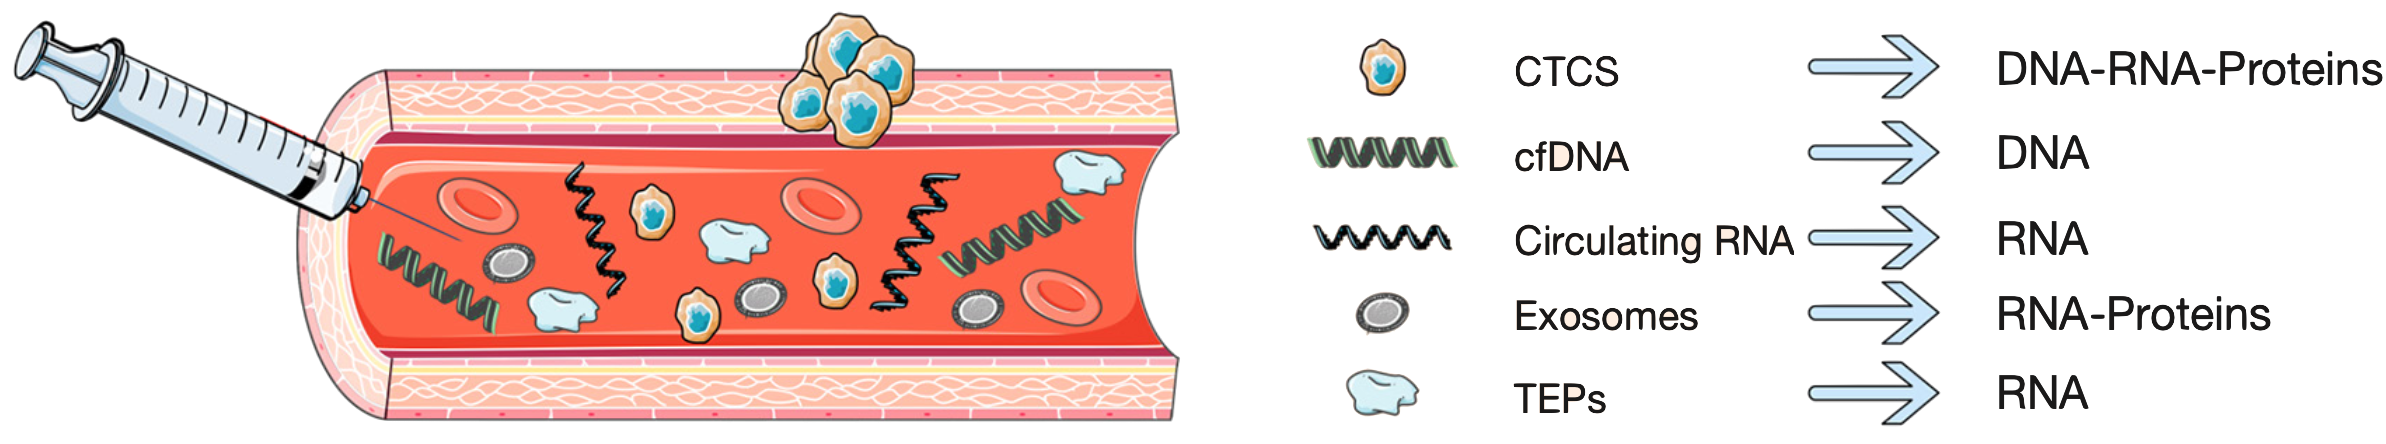
\includegraphics[width=\textwidth]{Images/chapter_1/liquid_biopsy.png}
    \caption{Tumor-derived components used as liquid biopsy biomarkers. Modified image from \cite{LB_ed}.}
    \label{fig:LB}
\end{figure}

\subsubsection{Circulating Tumor Cells (CTCs)}

CTCs are cancer cells that detach from the primary lesions or tumor metastases and then enter into the blood circulation. Specifically, these cells typically undergo an epithelial-mesenchymal transition (EMT) process, which allows them to enter the circulation and reach another remote target, where they undergo a reverse process called mesenchymal-epithelial transition (MET). Ultimately, this results in further cancer proliferation and therefore metastasis formation.

Although extremely rare, since only one CTC can be detected in an average of $10^6$–$10^7$ leukocytes, CTCs are found in around 50\% of patients affected by metastatic epithelial tumors and are used for the detection and monitoring of non-hematologic cancers \cite{CTC_prognosis, CTC_blood}. However, CTCs are fragile and thus require more complex laboratory procedures for isolation and enumeration, and the technology to characterize them is still evolving. Furthermore, the clinical significance of CTCs enumeration as a reliable diagnostic biomarker has yet to be established, although a high CTC count generally correlates with worse prognosis and metastatic spread of cancer \cite{CTC_prognosis}.

The CellSearch\textsuperscript\textregistered{} system is the most known U.S. FDA-approved CTC detection technology and it is capable of isolating CTCs with the use of anti-epithelial cell adhesion molecule (EpCAM) ferromagnetic beads.

\subsubsection{Circulating Tumor DNA (ctDNA)}

ctDNA is a single strand or double-stranded circulating free DNA (cfDNA) portion derived from apoptotic, necrotic, or living tumor cells that actively release DNA in the bloodstream by mechanisms not yet fully understood \cite{ctDNA}. 

Currently, several studies are investigating the association of ctDNA levels with tumor burden, tumor response, and survival outcome of lung cancer patients \cite{ctDNA, ctDNA_NSCLC}. However, since the absolute amount of ctDNA as a diagnostic tool is not significant, the attention has focused on real-time monitoring of tumor-specific genetic alterations to track the response to targeted therapies and drug resistance. In this context, novel and highly sensitive blood-based assays such as NGS and polymerase chain reaction-based techniques  (PCR), including digital PCR (dPCR), have emerged and are managing to overcome the problems of tumor DNA isolation and sequencing, which traditionally were slow and laborious processes. In fact, at present, it is possible to detect ctDNA even if it represents less than 1.0\% of the total cfDNA \cite{ctDNA_NSCLC, ctDNA_LB}.

ctDNA is now the most widely used biomarker for detecting genetic abnormalities in ALK-positive NSCLC patients. In this context, a positive finding of an actionable mutation in a cfDNA sample using PCR-based methods is enough to start or change a targeted treatment \cite{LB_NSCLC}.

\subsubsection{Exosomes}

Exosomes are cell-derived vesicles of endocytic origin with a diameter of 40–100 $nm$ that are released into the extracellular space and a variety of body fluids. They contain proteins as well as a range of nucleic acids, including DNA, mRNAs, and miRNAs, which are transferred to target cells, modulating their activities. In cancer they have a key role in metastatic niche preparation and cell-cell communication, favoring tumor growth, progression, and drug resistance \cite{Exosomes}. In addition, exosomes have a bilayer lipid membrane that protects nucleic acids, particularly RNAs, from ribonuclease degradation and extreme pH when found in body fluids. Therefore, there is a growing interest in these vesicles because their content could potentially serve as a biomarker in diagnosis, prognosis, and monitoring of the response to treatment \cite{LB_NSCLC, LB_atocha}. However, its isolation can be challenging.

Several techniques have been used for exosome isolation, such as density-gradient centrifugation, ultracentrifugation, and immunoaffinity methods based on the presence of specific protein markers, including CD63, CD9, and CD81 \cite{Exosomes}. Once isolated, they can be utilized to characterize the RNA and thus genetic alterations by using different techniques, including RT-PCR, nucleic acid sequencing, ELISE, or Western Blot. In summary, it is a promising source for analyzing EML4-ALK fusions, although its use in clinical practice has not yet been standardized. \cite{LB_atocha}.

\subsubsection{Tumor-Educated Platelets (TEPs)}

Platelets are the second most abundant cell type in peripheral blood and are known for their role in hemostasis. However, when they interact with tumor cells, they can undergo modifications, which will eventually affect tumor progression, dissemination, and establishment of an ideal environment for the proliferation of cancer \cite{Metastasis, Angiogenesis}. Specifically, this interaction induces the transference of tumor-associated biomolecules, including multiple RNA types and proteins, to platelets, resulting in the creation of TEPs.

When isolated, these platelets constitute a source of tumor RNA not only for NSCLC diagnosis but also for general molecular traces for cancer surveillance \cite{LB_atocha, Platelets}. Several methodologies have been used for platelet isolation and RNA profiling, although, as with exosomes, the complexities of these procedures are slowing their implementation in clinical routine. Currently, RNA transcripts could be quantified using microarray hybridization techniques, RT-PCR, or NGS. Therefore, in addition to exosomes, TEPs seem to have the potential to be used as liquid biopsy biomarkers for a variety of clinical and research applications, including the identification of fusion genes \cite{LB_atocha}.
    \chapter{Research Goals}

Diagnosis and targeting of ALK-positive NSCLC now form part of clinical routine, and the results obtained with ALK inhibitors are unprecedented considering the PFS and OS. However, although the development of novel drugs will continue to be a priority of cancer treatment, there is a need for better prognostic tools to assess therapeutic response, monitor tumor progression, and predict clinical outcomes.

In this context, the main objective of this thesis is to develop a new tool to better stratify patients, improving the current analysis of sequenced data from liquid biopsy samples. Eventually, this will allow oncologists to have more reliable information on the patient's tumor phenotype. Therefore, it will be possible to offer more individualized and optimal treatment to patients, without the risks associated with tissue biopsies.

This goal has led to the use in this study of non-invasive methods of describing tumor phenotype, including ctDNA and exosomes, to filter driver mutations in the ALK gene. Specifically, with the combination of molecular techniques and bioinformatics, this master's thesis aims to:
\begin{outline}
    \1 Establish analytical conditions for the study of mutations in the ALK gene from circulating DNA and exosomes in NSCLC advanced patients.
    \1 Perform a clinical study of mutations from circulating DNA and exosomes in a cohort of patients with advanced NSCLC.
    \1 Develop an automatic algorithm for filtering somatic mutations from sequenced data from ALK-positive NSCLC samples confirmed by PCR.
    \1 Estimate the utility of NGS and the developed algorithm for:
        \2 Detecting oncogenic drivers.
        \2 Identifying resistance mutations.
        \2 Monitoring therapy response.
        \2 Predicting clinical outcomes.
    \1 Assess the utility of liquid biopsy for the study of somatic mutations in the ALK gene from free circulating DNA and exosomes.
\end{outline}

    \chapter{Materials and Methods}

\section{Patient identification}


% The cohort for analysis was identified from an institutional database of NSCLC patients st st undergoing routine clinical tumor genotyping between January 1 , 2002 and January 1 , 2014.
% Patients were eligible if they consented to allow their clinical information to be used in retrospective research studies on an institutional review board (IRB)-approved protocol (Dana- Farber/Harvard Cancer Center protocol #02-180), or if they were deceased and data was made available on an IRB-approved waiver of consent. The database was queried for information on age, sex, race, smoking status, date of diagnosis, histology, stage, and date of death. Race was included given known associations between tumor genetics and patient race.


\section{Laboratory Procedures}

    \chapter{Results}

\section{Cohort of patients}

% TLCR
% Patients were followed from their diagnosis of stage IV disease.

% CCLM
% A total of 54 samples were obtained from 52 NSCLC patients and two healthy donors, after signing the appropriate informed consent.

% TESIS estela
% Para establecer la mejor estrategia metodológica, para la identificación del paciente candidato a recibir un inhibidor de ALK, se emplearán 20 muestras pre-tratamiento, pareadas de plasma y plaquetas, de pacientes con cáncer de pulmón no microcítico con enfermedad avanzada y translocación de ALK documentada según los protocolos asistenciales. Estas muestras se encuentran disponibles en el Biobanco del Hospital Universitario Puerta de Hierro.
% A fin de evaluar la utilidad de la biopsia líquida para monitorizar al paciente con translocación de ALK se reclutarán 30 pacientes, a razón de 15 pacientes por año. De cada paciente se recogerán muestras a los 2, 4, 6, 8, 12, 15 y 18 meses de tratamiento y a la progresión.
% % Los datos demográficos, clínico-patológicos, el estado mutacional del tumor, así como el estado funcional de los pacientes fueron obtenidos de los informes médicos. El ajuste de dosis y el cambio de medicación fueron documentados a lo largo del estudio.
%VARIABLES
% -Progresión de la enfermedad según criterios RECIST.
% -Supervivencia libre de progresión desde el inicio del tratamiento.
% -Supervivencia global desde el inicio del tratamiento.
% -Tasa de respuesta obtenida
% -Status EML4-ALK (positivo o negativo) en la biopsia líquida.
% -Niveles plasmáticos de EML4-ALK

% ALK paper
% In total, 33 plasma and 2 cerebrospinal fluid (CSF) specimens were collected and analyzed. Samples were collected at the time of disease progression which was assessed according to RECIST criteria v.1. 

\newpage

\section{Implemented Pipeline}

The development of the bioinformatic pipeline was divided into two steps: the implementation of the filtering algorithm itself; and that of a graphical interface to simplify the process of selecting parameters and saving the output variants with their properties in a \textit{.csv} file.

\subsection{Algorithm Characterization}

In order to detect all variants at the ALK gene locus, specific conditions for each type of them have been established from a set of previously validated samples. The flowchart in \autoref{fig:Algorithm} represents the basic structure of the developed pipeline and the selection criteria based on certain variables as presented in the \textit{non-filtered-oncomine.tsv} file.

\begin{figure}[ht]
    \centering
    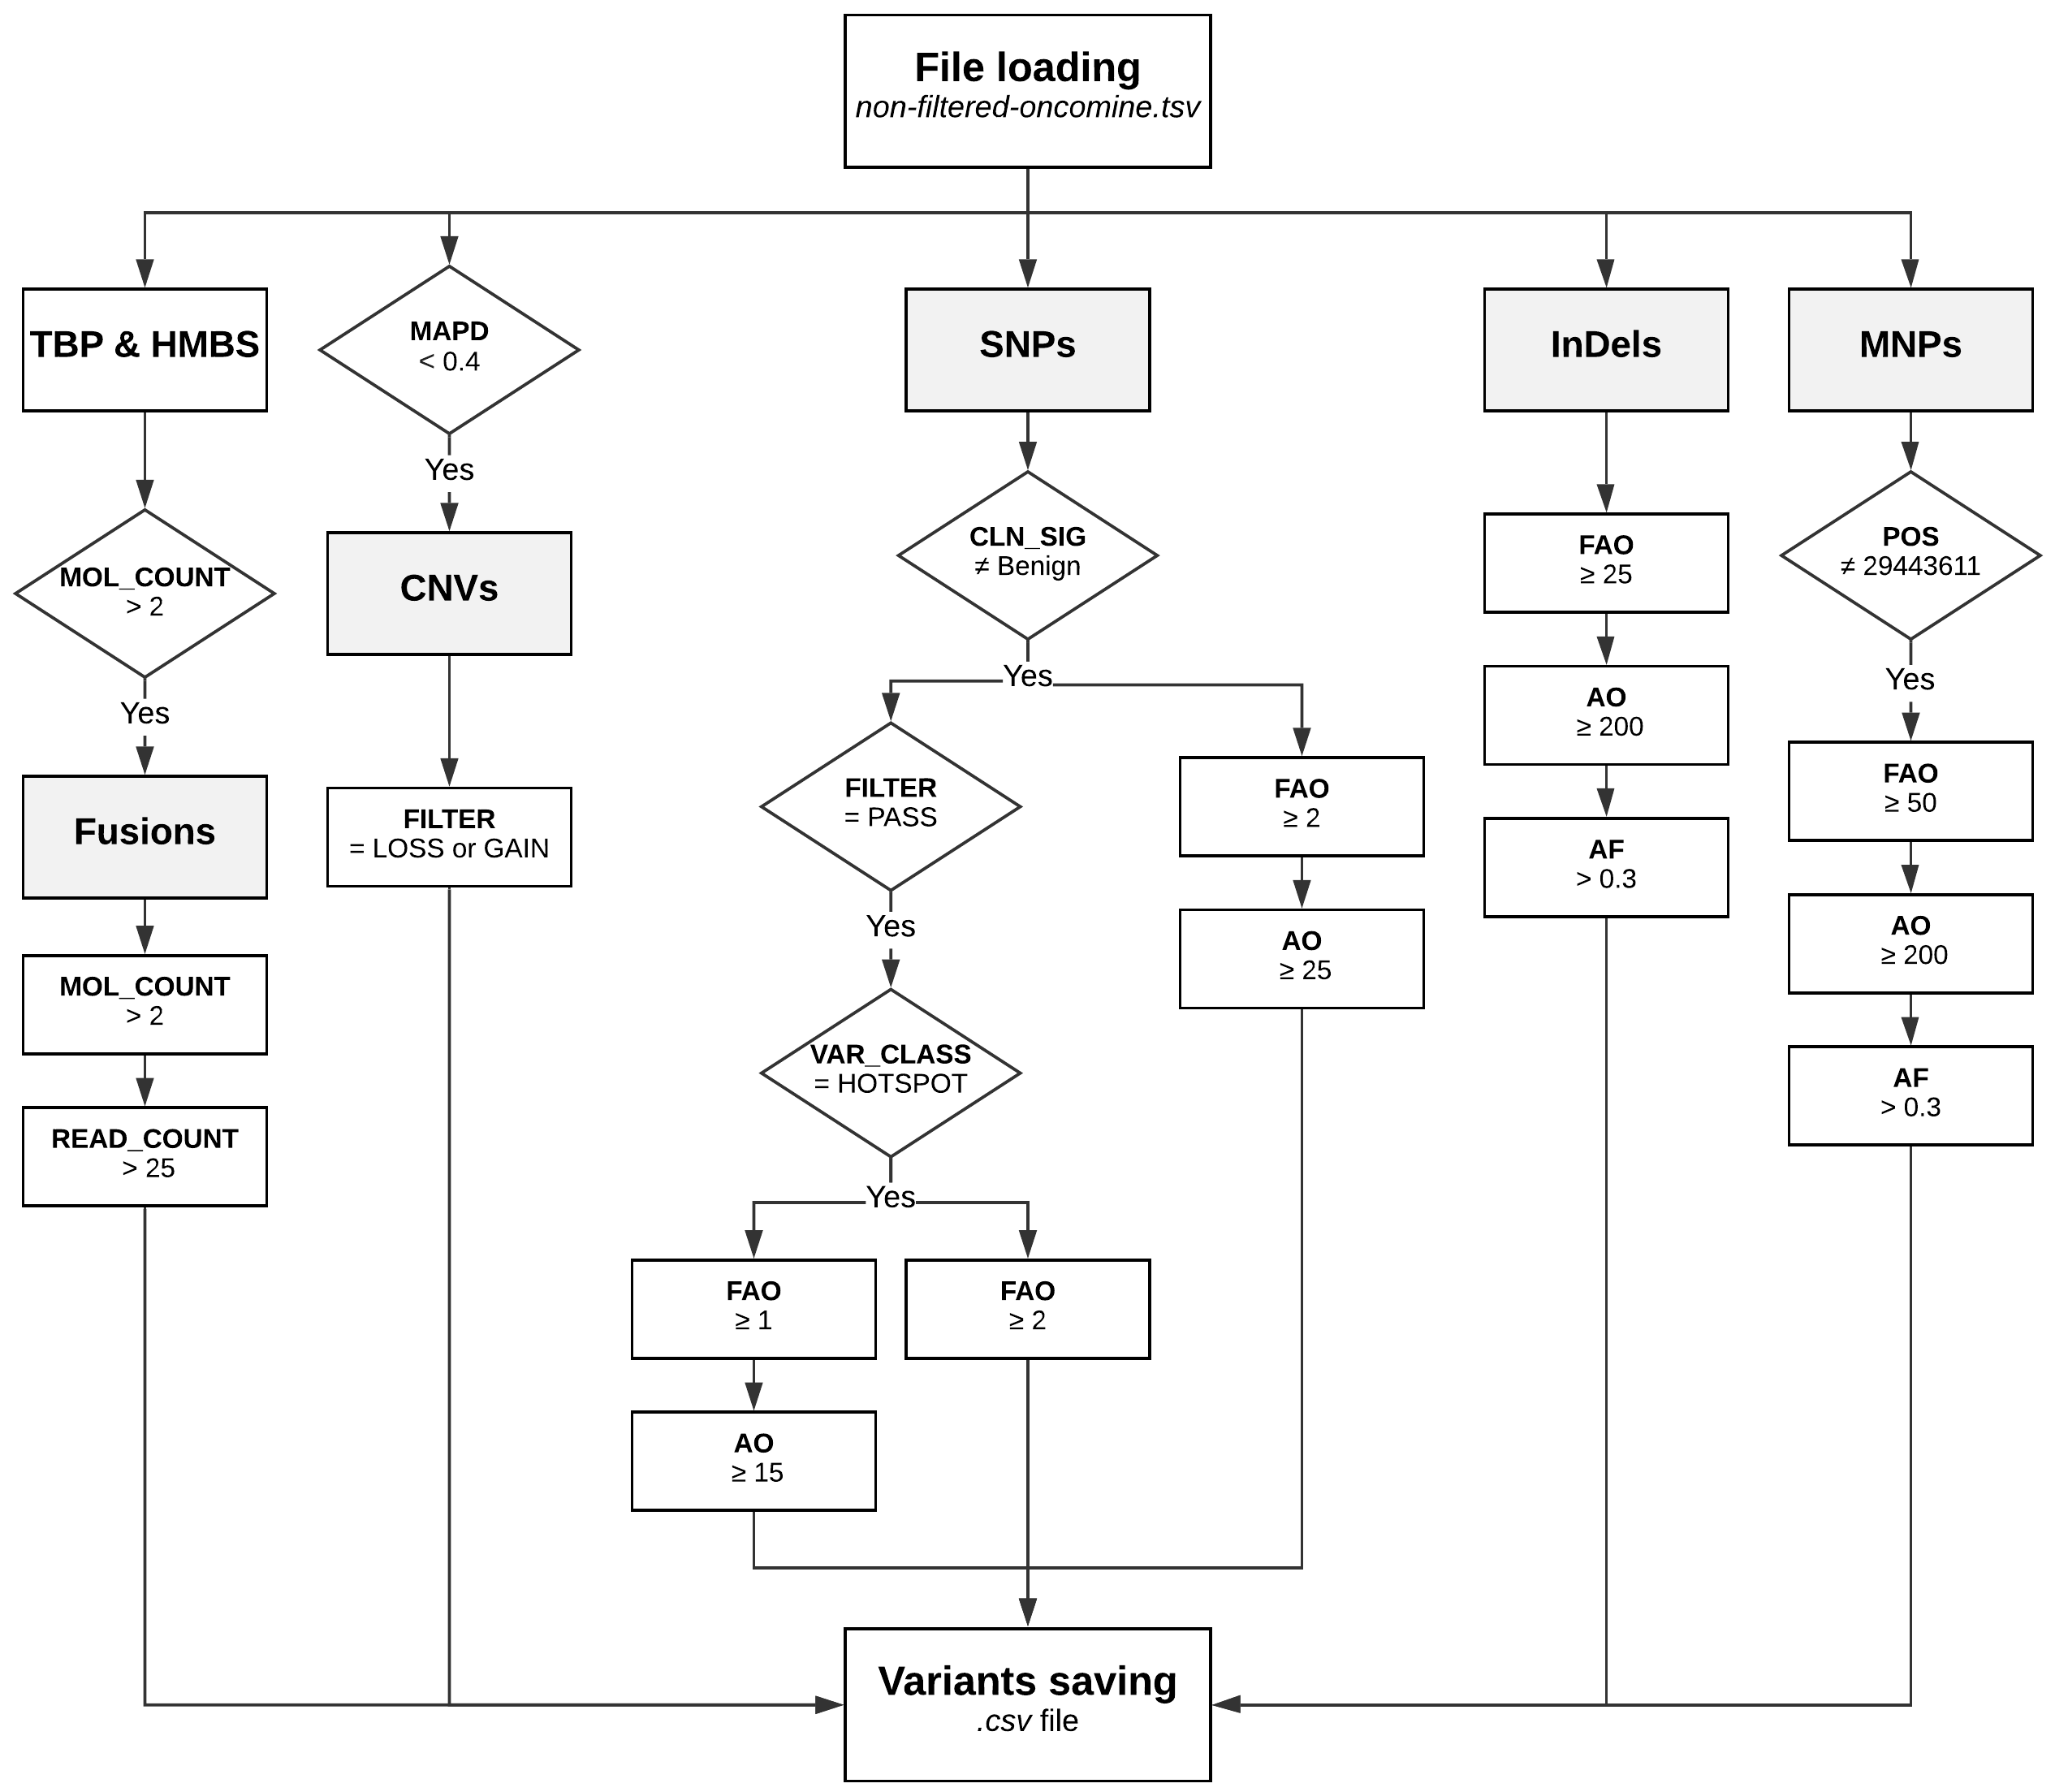
\includegraphics[width=\textwidth]{Images/chapter_4/mut_filtering.png}
    \caption{Flowchart of the bioinformatic pipeline optimized for the processing and assessment of variants at the ALK gene locus.}
    \label{fig:Algorithm}
\end{figure}

\subsubsection{Fusions Filtering}

The fusions filter selects translocations at the ALK locus with molecular coverage (MOL\_COUNT) $>$ 2, and fusion reads (READ\_COUNT) $>$ 25.

On the other hand, two control genes are included in each sequencing process to measure the transcript abundance, TATA-binding protein (TBP) and hydroxymethylbilane synthase (HMBS). Both must have molecular coverage (MOL\_COUNT) $>$ 2 to validate the filtered fusion variants by ensuring their correct amplification.

\subsubsection{Copy-Number Variations Filtering}

Following the Ion Reporter\texttrademark{} recommendations, to make a CNV call, the median of the absolute values of all pairwise differences (MAPD) must be $<$ 0.4. MAPD measures the absolute difference between the $log_2$ copy number ratios of adjacent amplicons and then calculates the median across all wells (\autoref{eq:MAPD}). Larger MAPD values indicate lower coverage uniformity and greater noise, resulting in a higher probability of erroneous CNV calls. Therefore, only samples showing an MAPD $<$ 0.4 were considered in further analysis, which consisted of selecting (FILTER) copy loss and gain in the ALK gene.
\begin{align} \label{eq:MAPD}
    MAPD &= median(\mid x_{i+1}-x_i \mid) \\
    \text{where}~  
    x_i &\equiv \text{$log_2$ ratio for marker i} \notag
\end{align}

\subsubsection{Single-Nucleotide Polymorphisms Filtering}

Taking into account that false positives of this type of variants are not common, the proposed algorithm makes a call as long as any of the following conditions is met, discarding variants with a benign or likely benign clinical significance (CLN\_SIG):
\begin{itemize}
    \item SNPs in hotspot regions (VAR\_CLASS) that have passed the Oncomine\texttrademark{} Variants v5.10 filter (FILTER) and that have been detected in at least 1 molecular count (FAO) with $\ge$ 15 reads (AO).
    \item SNPs in hotspot regions (VAR\_CLASS) that have passed the Oncomine\texttrademark{} Variants v5.10 filter (FILTER) and that have been detected in at least 2 molecular counts (FAO).
    \item SNPs that have been detected in at least 2 molecular counts (FAO) with $\ge$ 25 reads (AO).
\end{itemize}

\subsubsection{Insertions and Deletions Filtering}

The sequencing results usually present doubtful data regarding InDels. Therefore, the restrictions are more severe for this filter, which selects only variants that have been detected in at least 25 molecular counts (FAO) with $\ge$ 200 reads (AO) and an allele frequency (AF) $\ge$ 0.03.

\subsubsection{Multiple-Nucleotide Polymorphisms Filtering}

Based on data from confirmed ALK-positive samples, false positives are highly likely in MNPs. In this context, only variants that have been detected in at least 50 molecular counts (FAO) with $\ge$ 200 reads (AO) and an AF $\ge$ 0.03 were considered for confirmation by dPCR. 

On the other hand, abnormal Ion GeneStudio\texttrademark{} S5 Sequencer behavior at position chr2:29443611 of the ALK locus and involving the reading of 6 consecutive guanines (G) has been observed. Thus, variants of that location have been excluded from further analysis.

\subsection{Graphical User Interface (GUI)}

The implemented user interface has been developed to facilitate data input and interpretation of results.

\begin{figure}[ht]
    \centering
    \begin{subfigure}{\textwidth}
        \centering
        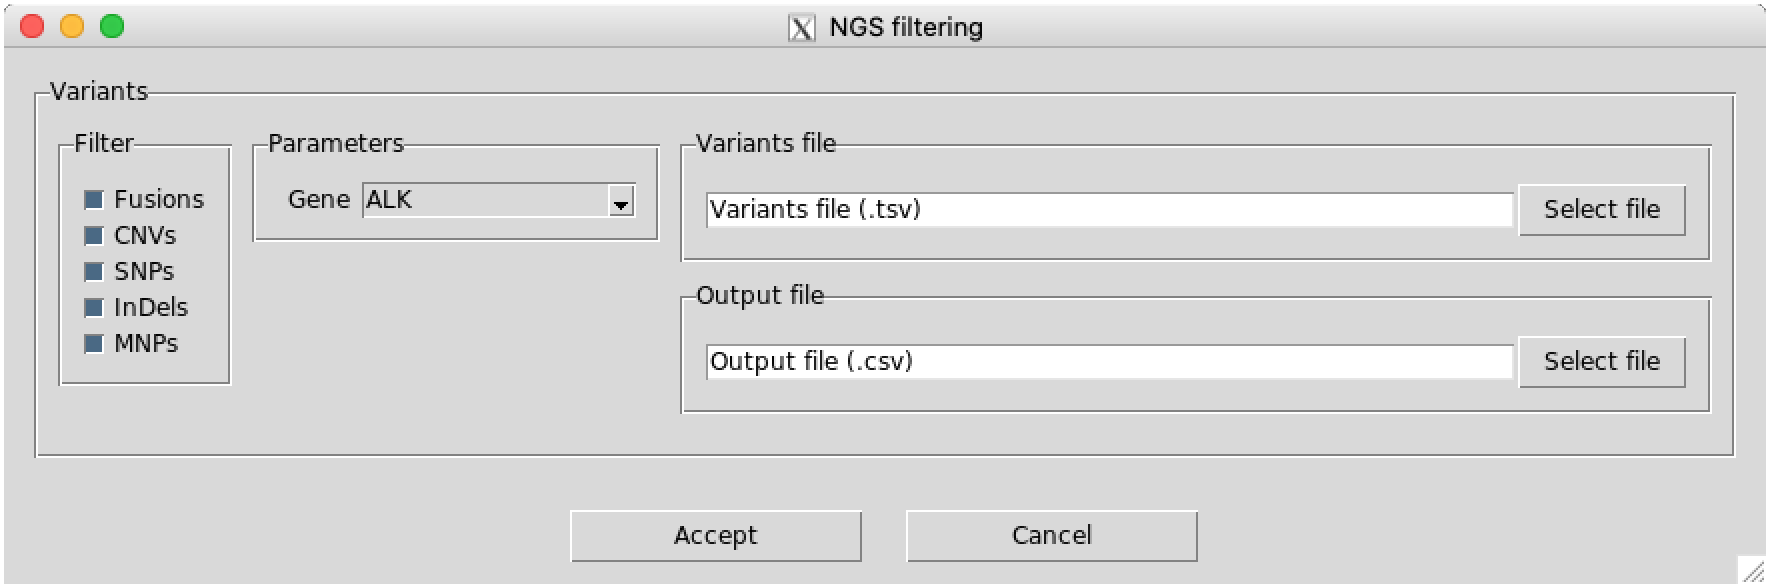
\includegraphics[width=\textwidth]{Images/chapter_4/GUI_1.png}
        \caption{GUI start screen. It allows selecting the type of variant\slash s to filter, the gene involved (ALK currently), as well as the source and output files. \\}
        \label{fig:GUI_1}
    \end{subfigure}
    \hfill
    \begin{subfigure}{0.47\textwidth}
        \centering
        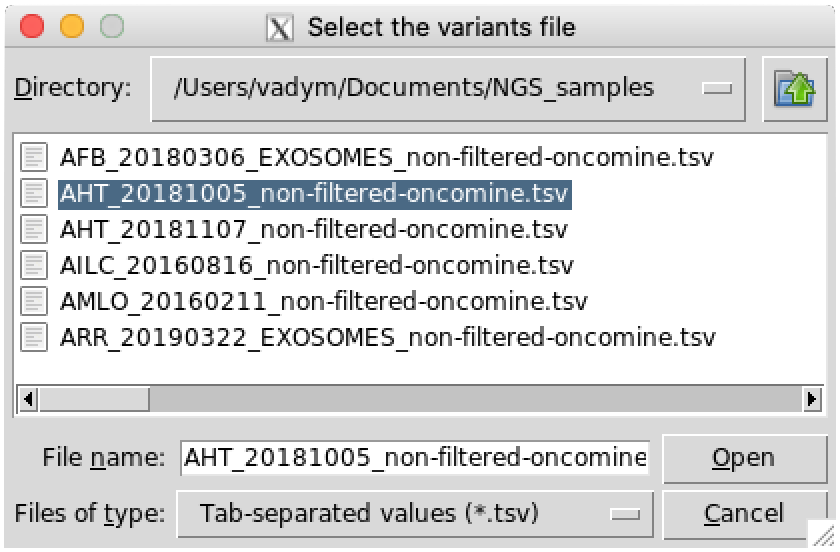
\includegraphics[width=\textwidth]{Images/chapter_4/GUI_2.png}
        \caption{GUI for selecting the \textit{.tsv} source file with the unfiltered variants.}
        \label{fig:GUI_2}
    \end{subfigure}
    \hfill
    \hfill
    \begin{subfigure}{0.52\textwidth}
        \centering
        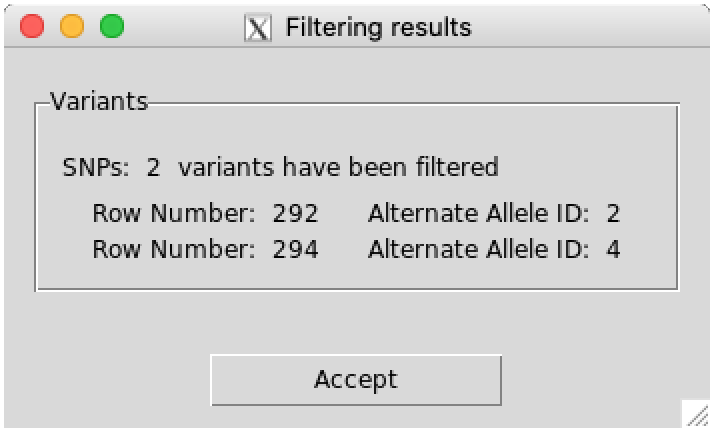
\includegraphics[width=\textwidth]{Images/chapter_4/GUI_3.png}
        \caption{GUI results screen showing 2 filtered SNPs and the properties that characterize them.}
        \label{fig:GUI_3}
    \end{subfigure}
    \hfill
    \caption{Implemented GUI that includes the entire filtering process.}
    \label{fig:GUI}
\end{figure}

As can be seen in \autoref{fig:GUI_1}, the start screen has several options that allow some variability when proceeding with the filtering process. On the one hand, it is possible to select the filter\slash s to apply to the \textit{non-filtered-oncomine.tsv} file, as well as the gene to study. Currently, and as previously described, only the ALK gene has been addressed. On the other hand, the user can select both the source and output files through a drop-down screen, which is shown in \autoref{fig:GUI_2}. In case the output file does not exist, the program creates it automatically.

Finally, to fully characterize the variants that have passed a particular filter, the results are displayed specifying the mutation type, the row number of the variants in the \textit{non-filtered-oncomine.tsv} file, and the ID of the alternate allele (\autoref{fig:GUI_3}). Simultaneously, each of the identified variants is appended to the output file along with its main characteristics.

It should also be noted that several additional screens have been implemented to offer the end-user information on the progress of the filtering process, on any errors that may have occurred during it, and on the non-identification of any variant of interest by the algorithm.

\section{Statistic Analysis}

% Análisis estadístico
% Los resultados de frecuencia se expresarán en términos absolutos, en porcentajes e intervalos de confianza y, las variables cuantitativas como media ± desviación estándar o mediana (rango) según proceda.
% Para evaluar la concordancia del status de la translocación (positivo/negativo) entre las muestras de sangre (plaquetas y plasma) pre-tratamiento y el tejido se empleará el coeficiente Kappa de Cohen y su intervalo de confianza. Además, se analizará la sensibilidad, especificidad, valor predictivo positivo y valor predictivo negativo de la detección de la translocación en plasma (exosomas) y plaquetas, tomando como gold standar el resultado del tejido.
% Para analizar los datos de supervivencia de los pacientes se tomará como fecha de inicio, la fecha de inicio al tratamiento en primera línea y se recabarán los datos de: fecha de progresión, de muerte o fecha de última visita al oncólogo. La supervivencia libre de progresión se calculará desde la fecha de inicio al tratamiento en primera línea. Para el análisis de PFS y SG se usará el método de Kaplan-Meier y como estadístico de contraste se usará el Log- Rank. Los valores de los HR obtenidos serán ajustados por las variables clínico-patologícas pertinentes.
%Las pruebas con un valor de p <0.05 serán consideradas estadísticamente significativas.
    \chapter{Discussion and Conclusions}

\section{Conclusions}

\section{Future Directions}

    %% This defines the bibliography file (main.bib) and the bibliography style.
%% If you want to create a bibliography file by hand, change the contents of
%% this file to a `thebibliography' environment.  For more information 
%% see section 4.3 of the LaTeX manual.
\begin{singlespace}
\bibliography{Bibliography/main}
\addcontentsline{toc}{chapter}{References}
\bibliographystyle{IEEEtran}
\end{singlespace}

    % \appendix
    % \chapter{Ethical, Social, Economic and Environmental Implications}

% ucm-t29753.pdf
% La investigación en el ámbito hospitalario

\section{Introduction}

\section{Impacts}

\subsection{Ethical impact}

\subsection{Social impact}

\subsection{Economic impact}

\subsection{Environmental impacts}

\section{Conclusions}

\clearpage
\newpage
    % \chapter{Budget}

\clearpage
\newpage
    % \include{Appendices/example_a}
    % \include{Appendices/example_b}
\end{document}
